%---------
% Thesis requirement: 10k ~ 15k words
%----------------------------------------------------------------------------------------
%	PACKAGES AND OTHER DOCUMENT CONFIGURATIONS
%----------------------------------------------------------------------------------------
% arara: xelatex: { shell: yes, synctex: yes }
%TC: ignore
\documentclass[
11pt, % The default document font size, options: 10pt, 11pt, 12pt
%oneside, % Two side (alternating margins) for binding by default, uncomment to switch to one side
english, % ngerman for German
singlespacing, % Single line spacing, alternatives: onehalfspacing or doublespacing
% draft, % Uncomment to enable draft mode (no pictures, no links, overfull hboxes indicated)
%nolistspacing, % If the document is onehalfspacing or doublespacing, uncomment this to set spacing in lists to single
%liststotoc, % Uncomment to add the list of figures/tables/etc to the table of contents
%toctotoc, % Uncomment to add the main table of contents to the table of contents
parskip, % Uncomment to add space between paragraphs
%nohyperref, % Uncomment to not load the hyperref package
headsepline, % Uncomment to get a line under the header
%chapterinoneline, % Uncomment to place the chapter title next to the number on one line
%consistentlayout, % Uncomment to change the layout of the declaration, abstract and acknowledgements pages to match the default layout
table
]{MastersDoctoralThesis} % The class file specifying the document structure
%TC: endignore
%TC:insert [\documentclass{book}]
\usepackage{soulutf8}
\usepackage{ifdraft}
\usepackage{tabularx, threeparttablex}
%  makecell
\usepackage{multirow}
\usepackage{array}
\usepackage{amsmath}
\usepackage{color}
% \usepackage{xcolor}
\usepackage{caption}

\newcommand{\drafting}{Draft Alpha}
% \renewcommand{\rothead}[2][60]{\makebox[9mm][c]{\rotatebox{#1}{\makecell[c]{#2}}}}
\ifdefined\drafting
\overfullrule=1mm

\else
\fi

\newcommand{\mc}{\multicolumn}
\newcommand{\mr}{\multirow}

\newcommand{\association}{\emph{association} }
\newcommand{\similarity}{\emph{similarity} }

% \newcolumntype{L}[1]{>{\raggedright\arraybackslash}p{#1}}
\newcolumntype{L}{>{\raggedright\arraybackslash}X}
\newcolumntype{R}{>{\raggedleft\arraybackslash}X}

% \usepackage[utf8]{inputenc} % Required for inputting international characters
\usepackage[T1]{fontenc} % Output font encoding for international characters
\usepackage{float}
\usepackage{mathpazo} % Use the Palatino font by default
\usepackage{datetime}
\usepackage[backend=biber,style=authoryear,natbib=true]{biblatex} % Use the bibtex backend with the authoryear citation style (which resembles APA)

\addbibresource{zotero_synced.bib} % The filename of the bibliography

\usepackage[autostyle=true]{csquotes} % Required to generate language-dependent quotes in the bibliography


%----------------------------------------------------------------------------------------
%	MARGIN SETTINGS
%----------------------------------------------------------------------------------------

\geometry{
	paper=a4paper, % Change to letterpaper for US letter
	inner=2.5cm, % Inner margin
	outer=3.8cm, % Outer margin
	bindingoffset=.5cm, % Binding offset
	top=1.5cm, % Top margin
	bottom=1.5cm, % Bottom margin
	% showframe, % Uncomment to show how the type block is set on the page
}

%----------------------------------------------------------------------------------------
%	THESIS INFORMATION
%----------------------------------------------------------------------------------------

\thesistitle{Similarity and Association: \\Principles of Distributed Semantic Processing in the Human Brain} % Your thesis title, this is used in the title and abstract, print it elsewhere with \ttitle
\supervisor{Sabine \textsc{Ploux}} % Your supervisor's name, this is used in the title page, print it elsewhere with \supname
\examiner{} % Your examiner's name, this is not currently used anywhere in the template, print it elsewhere with \examname
\degree{\href{http://sapience.dec.ens.fr/cogmaster/www/}{Research Master in Cognitive Sciences}} % Your degree name, this is used in the title page and abstract, print it elsewhere with \degreename
\author{Songsheng \textsc{Ying}} % Your name, this is used in the title page and abstract, print it elsewhere with \authorname
\addresses{} % Your address, this is not currently used anywhere in the template, print it elsewhere with \addressname

\subject{Cognitive Sciences} % Your subject area, this is not currently used anywhere in the template, print it elsewhere with \subjectname
\keywords{Lexical Semantics, fMRI, } % Keywords for your thesis, this is not currently used anywhere in the template, print it elsewhere with \keywordnames
\university{\href{https://www.ens.fr/en}{Ecole Normale Supérieure} \\ \href{https://www.parisdescartes.fr/en/homepage/}{Université Paris Descartes} \\ \href{https://www.ehess.fr/en}{Ecole des Hautes Etudes en Sciences Sociales}} % Your university's name and URL, this is used in the title page and abstract, print it elsewhere with \univname
\department{CNRS-EHESS} % Your department's name and URL, this is used in the title page and abstract, print it elsewhere with \deptname
\group{\href{http://cams.ehess.fr/the-cams/}{Centre for Social Analysis and Mathematics}} % Your research group's name and URL, this is used in the title page, print it elsewhere with \groupname
\faculty{\href{http://faculty.university.com}{Faculty Name}} % Your faculty's name and URL, this is used in the title page and abstract, print it elsewhere with \facname

\AtBeginDocument{
\hypersetup{pdftitle=\ttitle} % Set the PDF's title to your title
\hypersetup{pdfauthor=\authorname} % Set the PDF's author to your name
\hypersetup{pdfkeywords=\keywordnames} % Set the PDF's keywords to your keywords
}


% Define some commands to keep the formatting separated from the content 
\newcommand{\keyword}[1]{\textbf{#1}}
\newcommand{\tabhead}[1]{\textbf{#1}}
\newcommand{\code}[1]{\texttt{#1}}
\newcommand{\file}[1]{\texttt{\bfseries#1}}
\newcommand{\option}[1]{\texttt{\itshape#1}}

\begin{document}
%% TC:ignore
\frontmatter % Use roman page numbering style (i, ii, iii, iv...) for the pre-content pages

\pagestyle{plain} % Default to the plain heading style until the thesis style is called for the body content

%----------------------------------------------------------------------------------------
%	TITLE PAGE
%----------------------------------------------------------------------------------------

\begin{titlepage}
\begin{center}

\vspace*{.06\textheight}
{\scshape\LARGE \univname\par}\vspace{1.5cm} % University name
\textsc{\Large Master Thesis}\\[0.5cm] % Thesis type

\HRule \\[0.4cm] % Horizontal line
{\huge \bfseries \ttitle\par}\vspace{0.4cm} % Thesis title
\HRule \\[1.5cm] % Horizontal line
 
\begin{minipage}[t]{0.4\textwidth}
\begin{flushleft} \large
\emph{Author:}\\
\href{https://nicolasy.tk}{\authorname} % Author name - remove the \href bracket to remove the link
\end{flushleft}
\end{minipage}
\begin{minipage}[t]{0.4\textwidth}
\begin{flushright} \large
\emph{Supervisors:} \\
\href{http://cams.ehess.fr/sabine-ploux/}{\supname}\\ % Supervisor name - remove the \href bracket to remove the link  
\href{http://cams.ehess.fr/laurent-bonnasse-gahot/}{Laurent \textsc{Bonnasse-Gahot}}
\href{http://www.pallier.org/pages/cv.html#cv}{Christophe \textsc{Pallier}}
\end{flushright}
\end{minipage}\\[2cm]

\vfill

\large \textit{A thesis submitted in fulfillment of the requirements\\ for the degree of }\\
\large \textit{\degreename}\\[0.5cm] % University requirement text
\textit{Research project executed in the}\\[0.4cm]
\groupname\\\deptname\\[2cm] % Research group name and department name
 
\vfill

{\large \today}\\[3cm] % Date
%\includegraphics{Logo} % University/department logo - uncomment to place it
 
\vfill
\end{center}
\end{titlepage}

\ifdefined\drafting
%----------------------------------------------------------------------------------------
%	VERSION CONTROL
%----------------------------------------------------------------------------------------
	\vspace*{0.2\textheight}
	\drafting

	Compiled on
	\noindent \today, \currenttime
	\bigbreak

	\hfill YING
\else
\fi
%% TC:break [declaration]
%----------------------------------------------------------------------------------------
%	DECLARATION ORIGINALITY PAGE
%----------------------------------------------------------------------------------------
\ifdefined\drafting
\else
\begin{declarationauthorship}
    \addchaptertocentry{Declaration of Originality} % Add the declaration to the table of contents
    \noindent This master's project consists of an original research on the dissociation of multiple organization principles of human semantic processing. Namely, we relate various language-related cortical areas with different semantic functions using an fMRI encoding experiments. 
    
    This study differs from existing works in computational linguistics in the following points.
    \begin{itemize}
    \item It attempts to build non-generic semantic word embeddings, targeting specific semantic principles parallel to the paradigmatic and syntagmatic axes. Thus it requires fine tuning certain parameters when configuring existing embedding generation algorithms.
    \item Mathematic operations are applied on different types of semantic spaces to extract new embedding spaces. These manipulations show interactions between different embeddings.
    \item New baseline benchmark datasets are made available for French word-pair semantic proximity evaluation.
    \end{itemize}
    
    This study further investigates current theories and discoveries on a hypothetical function locus of semantic processing and multiple cortices' contribution in verbal comprehension with fMRI data.
    \begin{itemize}
    \item Existing works in semantic fMRI encoding either use non-ecological stimuli to reveal semantic condition contrasts, or ecological stimuli to reveal general semantic processing without targeting different (hypothetical) semantic aspects.
    \item A possible construction of \similarity and \association semantic memories are proposed and tested, which is based on converging evidences and theories on paradigmatic axis/semantic hub/convergence zone and syntagmatic axis/ associational activation.
    \item The anterior temporal lobe localization hypothesis for a central semantic processing component is tested with ecological fMRI encoding.
    \item This is the first project analyzing French fMRI data collected in the project ``Neural Computational Models of Natural Language'' (PI: John Hale and Christophe Pallier). Precedent projects were performed with English data.
    \end{itemize}
    
    The fMRI encoding pipeline also differs from most other works in the following aspects.
    \begin{itemize}
    \item When training voxel-models for BOLD prediction, a large grid-search for best regression parameters is carried out so that each voxel is modeled by the most appropriate functional features. 
    \item Multiple condition contrasting methods are employed including nested-model improvement testing and non-nested model performance comparison.
    \end{itemize}

    \end{declarationauthorship}
    
    \clearpage
\fi

\ifdefined\drafting
\begin{declarationcontribution}
    \addchaptertocentry{\contributionname} % Add the declaration to the table of contents
    \noindent I, \authorname (\textbf{SY}), declare that this Master's thesis titled, \enquote{\ttitle} and the work presented in it could not been accomplished without the help from the advisors of my research internship: Sabine \textsc{Ploux} (\textbf{SP}), Laurent \textsc{Bonnasse-Gahot} (\textbf{LBG}) and Christophe \textsc{Pallier} (\textbf{CP}).
    
    \begin{itemize} 
    \item \textbf{SP} helped enormously with the initial research problem definition and hypothesis formulation. Together with \textbf{LBG} and \textbf{CP}, they've given a rich literature collection on the relevant domain including brain encoding/decoding, theories on paradigmatic/syntagmatic axes.
    \item \textbf{CP} and Snežana \textsc{Todorović} designed the MRI experiment, prepared audio stimuli, textual reference data and behavioral control procedures. \textbf{CP} preprocessed MRI data including data cleaning and normalization. 
    \item \textbf{SY} implemented automatic pipelines and realized a large part of rule-based and manual correction of transcribed fMRI stimuli lemmatisation and semantic space vocabulary alignment. \textbf{SP} helped the verification of the results.
    \item \textbf{SY} adopted multiple semantic model validation tasks and dataset, implemented the initial iteration of dataset translation and correction, which is perfected by \textbf{SP}.
    \item \textbf{SY} adapted publicly available algorithms and tested combinations of hyper-parameter configurations to build one of the semantic representation models.
    \item \textbf{LBG} and \textbf{SP} actively participated in the conception of semantic space dissociation algorithm, which is later implemented and tested by \textbf{SY}. 
    \item \textbf{SP} visually examined iterations of the resulting semantic embedding models and assured the their quality and coherence.
    \item \textbf{CP} shared the fMRI analysis code base developed by him and collaborators. This project heavily depended on the regressor generation, design matrix orthogonalization functions of the library. \textbf{CP} also shared the computed feature of acoustic energy. \textbf{SY} added upon the code base functions to perform nested GridSearch regressions, implemented multiple statistical tests and result visualization pipelines.
    \item \textbf{LBG} and \textbf{CP} actively participated in the analysis and interpretation of fMRI regression results. They also gave useful guidance on the utilization of \code{nilearn, nibabel, nistat} libraries and analytical procedures including statistical tests and ROI analysis.
    \item \textbf{SY} drafted the Master's thesis, which is attentively proofread by \textbf{SP}, who also gave thoughtful insights on psycholinguistic discussion of the obtained results. \textbf{LBG} offered countless redactional good-practice advice during the drafting, which helped shaping this thesis. 
    \end{itemize}
     
    \noindent Signed:\\
    \rule[0.5em]{25em}{0.5pt} % This prints a line for the signature
     
    \noindent Date:\\
    \rule[0.5em]{25em}{0.5pt} % This prints a line to write the date
    \end{declarationcontribution}
    
    \cleardoublepage
\else
\fi

\ifdefined\drafting
\else
%----------------------------------------------------------------------------------------
%	QUOTATION PAGE
%----------------------------------------------------------------------------------------

\vspace*{0.2\textheight}

\noindent\enquote{\itshape Thanks to my solid academic training, today I can write hundreds of words on virtually any topic without possessing a shred of information, which is how I got a good job in journalism.}\bigbreak

\hfill Dave Barry
\fi

%% TC:break [abstract]
\ifdefined\drafting
\else
%----------------------------------------------------------------------------------------
%	ABSTRACT PAGE
%----------------------------------------------------------------------------------------

\begin{abstract}
\addchaptertocentry{\abstractname} % Add the abstract to the table of contents
The Thesis Abstract is written here (and usually kept to just this page). The page is kept centered vertically so can expand into the blank space above the title too\ldots

\end{abstract}

\fi

\ifdefined\drafting
\else
\begin{acknowledgements}
    \addchaptertocentry{\acknowledgementname} % Add the acknowledgements to the table of contents
    \vfil
    Besides Sabine \textsc{Ploux}, Laurent \textsc{Bonnasse-Gahot} and Christophe \textsc{Pallier}'s enormous contribution to this project as supervisors, I am also grateful for their time, openness and willingness for discussion and enlightening pedagogy.
    
    Sincere acknowledgements to Sabine \textsc{Ploux}, Jialiang \textsc{Lu}, Jean-Pierre \textsc{Nadal}, Yang \textsc{Yang}, Xiaoqing \textsc{Jin}, Junyan \textsc{Li}, whose supports were crucial to make this research internship happen. 

    Thanks to François \textsc{Deloche} for frequent technical supports, hosting the student seminars and animating the office, to Laurent \textsc{Bonnasse-Gahot} in addition to his essential role as a supervisor, for setting up and maintaining the server, and to all the colleagues from the CAMS for having shared the corridor and offices and most importantly a delightful working ambiance throughout my internship.

    I would also like to show my appreciation to Yinhao \textsc{Zeng}, Jianghao \textsc{Liu}, Karim \textsc{Lasri}, Anfu \textsc{Tang}, and Enrique \textsc{Gomez} for being interested in the project and beared with my tedious yet improving explanations. 
\end{acknowledgements}

\cleardoublepage
\fi

\tableofcontents % Prints the main table of contents

\ifdefined\drafting
\else
\listoffigures % Prints the list of figures
\listoftables % Prints the list of tables
\fi


%----------------------------------------------------------------------------------------
%	ABBREVIATIONS
%----------------------------------------------------------------------------------------

\begin{abbreviations}{ll} % Include a list of abbreviations (a table of two columns)

    \textbf{BA} & \textbf{B}roadmann \textbf{A}rea \\
    \textbf{BOLD} & \textbf{B}lood-\textbf{O}xygen-\textbf{L}evel \textbf{D}ependent \\
    \textbf{CSC} & \textbf{C}ontrolled \textbf{S}emantic \textbf{C}ognition \\
    \textbf{CV} & \textbf{C}ross \textbf{V}alidation \\
    \textbf{EEG} & \textbf{e}lectro\textbf{e}ncephalo\textbf{g}raphy\\
    \textbf{ERP} & \textbf{E}vent \textbf{R}elated \textbf{P}otential \\
    \textbf{fMRI} & \textbf{f}unctional \textbf{M}agnetic \textbf{R}esonance \textbf{I}maging \\ 
    \textbf{GLM} & \textbf{G}eneral \textbf{L}inear \textbf{M}odel \\
    \textbf{MEG} & \textbf{m}agneto\textbf{e}ncephalo\textbf{g}raphy\\
    \textbf{PC} & \textbf{P}rinciple \textbf{C}omponent \\
    \textbf{PET} & \textbf{P}ositron \textbf{E}mission \textbf{T}omography \\
    \textbf{POS} & \textbf{P}art-\textbf{O}f-\textbf{S}peech \\
    \textbf{ROI} & \textbf{R}egion \textbf{o}f \textbf{I}nterest \\
    \textbf{SD} & \textbf{S}emantic \textbf{D}ementia \\
    \textbf{SDR} & \textbf{S}tatistical \textbf{D}istributed \textbf{R}epresentation Models \\
\addlinespace

\midrule           
\textbf{Embedding Spaces}\\
\midrule
\\
\textbf{SIM} & \textbf{SIM}ilarity \\ 
\textbf{SIG} & \textbf{SI}milarity projected on Dep\textbf{G}love \\
\textbf{ASN} & \textbf{AS}sociatio\textbf{N} \\
\textbf{MIX} & \textbf{MIX}ed \\
\end{abbreviations}

\ifdefined\drafting
\else
%----------------------------------------------------------------------------------------
%	PHYSICAL CONSTANTS/OTHER DEFINITIONS
%----------------------------------------------------------------------------------------

\begin{constants}{lr@{${}={}$}l} % The list of physical constants is a three column table

% The \SI{}{} command is provided by the siunitx package, see its documentation for instructions on how to use it

Speed of Light & $c_{0}$ & \SI{2.99792458e8}{\meter\per\second} (exact)\\
%Constant Name & $Symbol$ & $Constant Value$ with units\\

\end{constants}

%----------------------------------------------------------------------------------------
%	SYMBOLS
%----------------------------------------------------------------------------------------

\begin{symbols}{lll} % Include a list of Symbols (a three column table)

$a$ & distance & \si{\meter} \\
$P$ & power & \si{\watt} (\si{\joule\per\second}) \\
%Symbol & Name & Unit \\

\addlinespace % Gap to separate the Roman symbols from the Greek

$\omega$ & angular frequency & \si{\radian} \\

\end{symbols}
\fi

\ifdefined\drafting
\else
%----------------------------------------------------------------------------------------
%	DEDICATION
%----------------------------------------------------------------------------------------

\dedicatory{For/Dedicated to/To my\ldots} 
\fi
%----------------------------------------------------------------------------------------
%	THESIS CONTENT - CHAPTERS
%----------------------------------------------------------------------------------------
%% TC:endignore
%TC:break body
\mainmatter % Begin numeric (1,2,3...) page numbering

\pagestyle{thesis} % Return the page headers back to the "thesis" style

% Include the chapters of the thesis as separate files from the Chapters folder
% Uncomment the lines as you write the chapters

\chapter{Introduction} 

\label{chap:introduction} 

%----------------------------------------------------------------------------------------
\section{Semantic Memory, Representation and Processing} 

Semantics as in linguistic context, is the connection between language forms such as orthography, syntax, and meanings including lexical and phrasal ones. The brain processes semantics in aide of semantic memory \parencite{tulvingEpisodicSemanticMemory1972}, of which the loci in human cognition system are still actively being debated. 

Semantic memory is unlike episodic memory, which is individual-specific and modality dependent. As semantic memory is associated with general world knowledge \parencite{mcraeSemanticMemory2013}, semantic memory tends to be shared across individuals within a common cultural background. Such invariance provides a window for semantic memory loci localization in the human brain. 

In \citeauthor{tulvingEpisodicSemanticMemory1972}'s view, semantic memory is conceptually dissociated, but not necessarily functionally or structurally separated from procedural and episodic memory. However, studies \parencite{vargha-khademDifferentialEffectsEarly1997} suggest the structural and functional dissociation of episodic memory and semantic memory, and that parahippocamal cortices, as a classical theoretical locus of episodic memory, are not crucial for the normal functioning of semantic memory.

\begin{table}

\centering

\begin{tabularx}{\textwidth}{@{} L *{5}{X} @{}}
\toprule
\tabhead{Reference} & \tabhead{Frontal Lobe} & \tabhead{Temporal Lobe} & \tabhead{Parietal Lobe} & \tabhead{Occipital Lobe} & \tabhead{Limbic Lobe}\\
\midrule
\cite{tsukiuraDissociableRolesBilateral2006} & IFG & CA, STG & AG & GF & PCG \\
{[}TODO More weekend{]} &  &  &  &  &  \\
\bottomrule \\
\end{tabularx}
\caption{Involvement of Cerebral Areas in Semantic Tasks}
\label{tab:distributedareastudysynthesis}
\end{table}
    

While some theorist argue for the temporal localization of semantic memory~\parencite{saumierSemanticMemory2002, martinSemanticMemoryBrain2001}, recent studies found neural correlates of semantic knowledge distributed in multiple lobes (refer to Table \ref{tab:distributedareastudysynthesis} for a resume), supporting thus the distributed hypothesis that semantic knowledge might be encoded in multiple brain areas. The cortices involved in semantic processing other than the temporal cortex, are strongly associated to perceptual, sensorial and/or affectual functions, suggesting that semantic memory depends on episodic events~\parencite{moseleyNounsVerbsObjects2014}. 

A theoretical reconciliation between these two schools is the specialization of cortical areas implicated in semantic tasks: the abstract, amodal semantic memory being grounded by concrete modal episodic memories \parencite{pecherGroundingCognitionRole2005}. 

The classical semantic memory locus could serve as the convergence zone for binding information from modality-specific cortices \parencite{damasioNeuralBasisLexical1996, damasioNeuralSystemsWord2004, simmonsSimilarityintopographyPrincipleReconciling2003}. Anatomical evidences, that the possible loci sit at convergences of multiple perceptual processing streams \parencite{binderNeurobiologySemanticMemory2011}, support this theory. \textcite{pattersonWhereYouKnow2007} further exploited \citeauthor{damasioNeuralSystemsWord2004}'s arguments by proposing the \emph{Hub-and-Spoke} model, where a semantic hub, not only acts as a pointer and a information-binder, but also constructs, refines semantic concepts and builds cross-modal similarity structures using episodic event. In parallel, \textcite{paivioMindItsEvolution2008} argued for a dual-coding system to address the problem of representing abstract concepts which do not necessarily have perceptual input: in addition to accumulated perceptual information for concrete concepts, a more meta-semantic department keeps record for all concepts. 



In this project, we restrain the discussion to lexicosemantic system, particularly we will focus on the representation and processing of word meanings in an ecological auditive experiment. 

\section{Syntagmatic and Paradigmatic Axes in Linguistics}
\label{sec:IntroSyntagandParaAxies}
\textcite{jakobsonFundamentalsLanguage1963} and \textcite{desaussureCoursLinguistiqueGenerale1969} propose that all linguistic units are arranged in two modes which are \emph{combination} and \emph{selection}, or \emph{syntagm} and \emph{paradigm}. \emph{Combination} is in \emph{presentia} as the linguistic unit (in the current context, a word / lemma / lexicon unit) is contextualized by other elements presented in a linguistic sequence. \emph{Selection} is in \emph{absentia} as it is linked to other alternative substitutions which are absent from the current context. Table \ref{tab:egsyntagparadig} gives an example of the organization in two axes.

\begin{table}
    \centering
    \begin{ThreePartTable}  
    \begin{tabularx}{\textwidth}{p{3mm}p{1mm}*{7}{L}}
     & \multicolumn{7}{c}{\tabhead{syntagmatic}} \\
     \parbox[t]{1mm}{\multirow{7}{*}{\rotatebox[origin=c]{90}{\tabhead{paradigmatic}}}} & \tikzmark{ps} & \tikzmark{ss} &  &  &  & & &  \tikzmark{se} \\
    & & The & ridiculous & girl & fell & into & the & pond. \\
    & & & \textcolor{gray}{silly} & \textcolor{gray}{person} & \textcolor{gray}{jumped} & & & \textcolor{gray}{river.} \\
    & & & \textcolor{gray}{foolish} & \textcolor{gray}{woman} & \textcolor{gray}{tripped} & & & \textcolor{gray}{lake.} \\
    & & & \textcolor{gray}{funny} & \textcolor{gray}{lady} & \textcolor{gray}{plunged} & & & \textcolor{gray}{sea.} \\
    & & & \textcolor{gray}{crazy} & \textcolor{gray}{princess} & \textcolor{gray}{walked} & & & \textcolor{gray}{ocean.} \\
    & \tikzmark{pe} & & \textcolor{gray}{klutzy} & \textcolor{gray}{child} & \textcolor{gray}{ran} & &  & \textcolor{gray}{pool.} \\
    \end{tabularx}
    \end{ThreePartTable}
    \caption[Example of Syntagmatic and Paradigmatic Axes]{An example of syntagmatic and paradigmatic axes. Gray-colored texts are in \emph{absentia}, black-colored texts are in \emph{presentia}. \emph{Syntagm} combines word sequence into a meaningful sentence, while \emph{paradigm} provides feasible substitutions of currently-present words.\label{tab:egsyntagparadig}}
    \begin{tikzpicture}[overlay, remember picture, yshift=.25\baselineskip, shorten >=.5pt, shorten <=.5pt]
        \draw [->] ([yshift=.75pt]{pic cs:ps}) -- ({pic cs:pe});
        \draw [->] ([yshift=.75pt]{pic cs:ss}) -- ({pic cs:se});
      \end{tikzpicture}
\end{table}


\citeauthor{jakobsonFundamentalsLanguage1963} further illustrated the twofold character of language via selection-deficient and contexture-deficient aphasics using data from \textcite{goldsteinLanguageLanguageDisturbances1948, headAphasiaKindredDisorders1920, hughlingsjacksonAffectionsSpeechDisease1879, goldsteinProblemMeaningWords1971, luriaWorkingBrainIntroduction1976c, crutchAbstractConcreteConcepts2004, warringtonCategorySpecificAccess1983}, bridging formal linguistic works with psycholinguistic studies.

Similarity disorder (selection-deficiency) patients are able to complete scraps of words or sentence, but are unable to uncontextualize themselves, thus unable to utter ''it rains'' unless it rains actually. The retrieval of the most precise lexicon is blocked, and the internal relation between concepts are dissolved. For those patients, an isolated word means nothing, occurrences of one same word in different contexts are homonyms, and the production of word tends to be bound by other associative words (for example, \emph{knife} are referred to as \emph{pencil-sharpener}, \emph{bread-knife} and \emph{knife-and-fork}) or metonymies (\emph{fork} for \emph{knife}, \emph{eat} for \emph{toaster}), or replaced by the most general terms such as \emph{chose} and \emph{machin} in French. The utterances are highly dominated by spatial, temporal and usage proximities, which are not necessarily parallel to similarity. They also lose the ability to switch register and stay in their idiolect reality. As remarked by \citeauthor{jakobsonFundamentalsLanguage1963}, for such an aphasic whose substitutional capacity has been disabled and contextual capacity intact, the emissive and receptive linguistic competence relies solely on contiguity. 

Contiguity disorder (contexture-deficiency) patients, on the other hand, are impaired to propositionize, inflect and desolve compound words such as \emph{thanksgiving} into \emph{thanks} and \emph{giving}. They produce agrammatical sentences as a chaotic word heap. The approximative identifications of a presented concept are quasimetaphoric (such as \emph{spyglass} are produced for \emph{microscope}, \emph{fire} for \emph{gaslight}), without any deliberate transfer of meaning as it is in the case of poetry and rhetorics. 

%----------------------------------------------------------------------------------------

\section{Computational Semantic Representation Modeling}

Natural language processing and understanding in general artificial intelligence has partially branched away from cognitive computational linguistic works. While language representation models like BERT~\parencite{devlinBERTPretrainingDeep2018} are fine-tuned to natural language processing benchmark tasks, they do not necessarily approach human language processing. We restrain computational semantic modeling to the models attempting to replicate of human linguistic dynamics. 

Semantic representation models digitalize the natural language word meanings into numeric representations that can be understood and processed by neural networks and computer systems. There are two schools of modeling: symbolic and distributional.

\subsection{Symbolic Relational Semantic Models}

\label{subsection:symbolicembedding}
Classical semantic models assumes the meanings can be considered as an indexable binary feature array \parencite{smithSemanticMemoryPsychological1974} or interconnected nodes in a large semantic graph-like ontological network \parencite{collinsRetrievalTimeSemantic1969}. In such structures, the binary features and nodes in the ontologies each represents a semantic entity (\emph{symbol}), to which we associate properties or values. Depending on the implementation, such symbolic structures are usually abstracted or independent from episodic, perceptual experiences. They are able to account for abstract taxonomical conceptual comparisons. Therefore, they model mainly paradigmatic similarities. 

Modern implementation of such models still rely largely on human manual coding. WordNet-alike knowledge bases \parencite{millerWordNetLexicalDatabase1995, millerWordNetElectronicLexical1998, sagotBuildingFreeFrench2008, pradetWonefImprovedExpanded2014} are examples of symbolic semantic networks which encodes inter-word semantic relations. In this class of models, lexicon units are regrouped into \emph{synsets}, forming synonymy sets, each representing one different meaning of the unit. Synsets are interconnected with relations such as \emph{antonymy, hyponymy, hypernymy, meronymy, toponymy}\dots

\subsection{Statistical Distributed Representations}

\label{subsection:statisticalembedding}

\textcite{harrisDistributionalStructure1954}'s distributional hypothesis argues that ``linguistics items with similar distributions have similar meanings.'' Most statistical models based on this theoretical foundation could be classified into latent semantic inference models \parencite{deerwesterUnitedStatesPatent1989, penningtonGloveGlobalVectors2014} and hyperspace analogue to language models \parencite{burgessHyperspaceAnalogueLanguage1995, mikolovEfficientEstimationWord2013, levyDependencyBasedWordEmbeddings2014}. As they make heavy use of contextual information, the syntagmatic information are also present those classes of models.

Such representation models use high dimensional vectors to encode semantic entities. The 2D matrix representation of the model, where the rows are entries of the lexicon, columns being the vector dimensions, are referred to as \emph{semantic embeddings} or \emph{semantic spaces}. Similarity measures are derived on vector distance metrics including cosine distance, gaussian distance and Minkowski distances. Models such as \textcite{penningtonGloveGlobalVectors2014, mikolovEfficientEstimationWord2013} successfully capture semantic information from textual statistics, achieving adequate performance on similarity benchmarks. 

On the linguistic nature of statistical distributed representation (SDR) models, we observed a mixture of syntagmatic and paradigmatic information in statistical embeddings. To give an example, in an openly available GloVe~\parencite{penningtonGloveGlobalVectors2014} implementation\footnote{Wikipedia 2014 + Gigaword 5 with 6B tokens, 400k uncased vocabulary and 300 dimensions. \url{https://nlp.stanford.edu/projects/glove/}.}, the closest neighbors of the target word \emph{teacher} (a noun) are composed of synonyms (\emph{instructor, tutee}) and associates (\emph{classroom, teaching, school, student, aunt\dots}) (Table \ref{tab:gloveneighbours}).  While the list of synonyms proposed by WordNet is \emph{instructor, teaching fellow, docent, coach}, which is purely paradigmatic.


\begin{table}
    \centering
    \begin{ThreePartTable}  
    \begin{tabularx}{\textwidth}{*{4}{L}}
    \multicolumn{2}{l}{\tabhead{Target word:}} & teacher & \\
    \toprule
    \tabhead{Neighbour} & \tabhead{Cosine Distance\tnote{1}} & \tabhead{Nature of Neighbour} & \tabhead{Semantic Relation} \\
  \toprule
classroom & 0.537 & associate & locative \\
teaching & 0.497 & associate & action \\
school & 0.484& associate & locative \\
preschool & 0.453 & associate & locative \\
student & 0.421& associate & object/agent\\
grade & 0.418 & associate & \\
college & 0.403 & associate & locative \\
instructor & 0.401 & synonym & \\

    \bottomrule
    \end{tabularx}
    \begin{tablenotes}
        \footnotesize
        \item[*] A cosine distance near 0 indicates a greater similarity.
    \end{tablenotes}  
    \end{ThreePartTable}
    \caption[Example of Syntagmatic and Paradigmatic Mixture in Statistical Semantic Models]{\emph{Teacher} are judged to be close to \emph{classroom, teaching, student}\dots. While they are frequent collocations, they are nevertheless not synonyms. \label{tab:gloveneighbours}}
\end{table}

\textcite{lapesaContrastingSyntagmaticParadigmatic2014} tested combinations of different hyper-parameters of co-occurrence-based statistical representation building algorithm. They used behavioral priming data of syntagmatic and paradigmatic word-pairs to contrast parameters' influence on two axes' performance. Figure \ref{fig:synparacontextwindow} is reproduced using the reported data from the work, confirming more systematically the two-fold mixture in SDR embeddings.

\begin{figure}
    \centering
    \makebox[\linewidth]{
    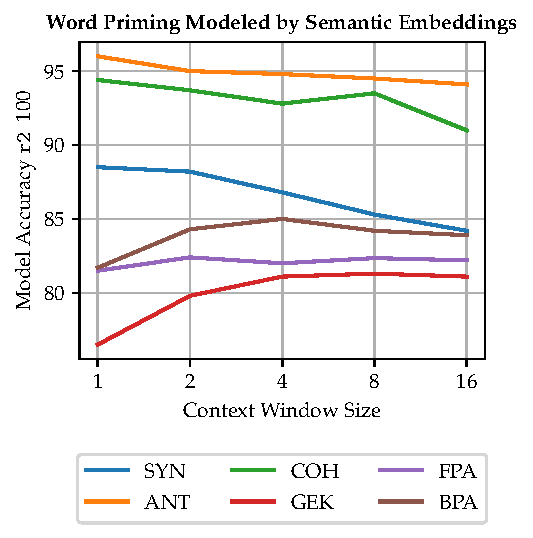
\includegraphics[scale=1]{Figures/SynParaContextWindow.pdf}
    }
    \caption[Impact of Context Window Size on Syntagmatic and Paradigmatic Information Extraction]{\textcite{lapesaContrastingSyntagmaticParadigmatic2014} tested 6 priming scheme datasets: paradigmatic datasets include synonyms \code{SYN}, antonyms \code{ANT} and cohypernyms \code{COH}, syntagmatic datasets include forward phrasal associates \code{FPA}, backward phrasal associates \code{BPA} and generalized event knowledge \code{GEK}. For each of the 6 datasets, they trained a separate GLM using differently configured semantic embeddings to predict word priming delays. Increasing context window size when training the embedding improves syntagmatic model accuracy, while penalizes paradigmatic predictions. Note that paradigmatic results are consistently better than syntagmatic ones.} 
    \label{fig:synparacontextwindow}
\end{figure}


%----------------------------------------------------------------------------------------

\section{Semantic Neural Encoding/Decoding Experiments}

The cognitive account of semantic processing includes the identification of the specific functions of various cortical areas during the semantic process. Historically, neuroscientists had to rely on semantic deficits and lesion studies. With cognitive modeling development, neuroimaging techniques enabled the examination of various model proposals without having to open the skull. 

\textcite{marrVisionComputationalInvestigation1982} proposed the three levels of modeling in: \emph{computation, algorithm} and \emph{implementation}. On operating on the computational level, cognitive modelers either try to replicate the temporal-spatial dynamics of cerebral activities, thus \emph{encodes} neural signals, and/or use measured signals to recover external stimuli, thus \emph{decodes} brain activity. 

Given the temporal and spatial resolution constraints of neuroimaging techniques among electroencephalography (EEG), magnetoencephalography (MEG), functional magnetic resonance imaging (fMRI), positron emission tomography (PET), fMRI and PET gained enormous popularity in the semantic localization studies while MEG for spatial-precise temporal dynamic studies~\parencite{molloOscillatoryDynamicsSupporting2017}. fMRI gives a much better spatial resolution than EEG (up to millimeters), but it is generally poor in temporal resolution. Classic semantic stimuli units are presented at sub-second level (hundreds of milliseconds) but the usual imaging frequency is at second level, and the measured blood-oxygen-level dependent (BOLD) signal approximates a temporal convolution of real neuron activation and hemodynamic function over 4 to 7 seconds.

Encoding and decoding experiments heavily rely on computational semantic representation models, especially distributed representations. \textcite{mitchellPredictingHumanBrain2008} was the first work to use contextual co-occurrence vectors (one variate of SDR) to encode semantic processing activities for concrete nouns. The predictive model showed significant generalization power, indicating a strong association between semantic embeddings and the brain activity, and the feasibility of encoding fMRI recorded semantic brain activity.

\subsection{Multi-Network Participation in Semantic Processing}
\label{subsec:multinetworkParticipation}
A large amount of literatures with encoding and decoding experiments report results in favor of distributed semantic processing in the human brain. 

\textcite{mitchellPredictingHumanBrain2008}'s concrete noun encoding experiments reported the most accurately predicted voxels to be located in (pre)frontal, parieto-temporal regions. \textcite{pereiraUniversalDecoderLinguistic2018} used fMRI signals to decode lexical and phrasal semantic stimuli presented in isolation. Among the 5000 most informative voxels found for each subject, functional networks in human brain other than the linguistic one take also a significant portion consistently across subjects. 

In addition to experiments conducted with isolated semantic stimuli, works such as \textcite{todorovicAnalysesIRMfLors2018, verdierEncodageActiviteNeuronale2018} [TODO, add more refs] experimented with ecological stimuli. They found consistent encoding / decoding performance with non-classically-linguistic cortical area voxels.

Multiple theories exist to account for the contribution of other cortical areas in semantic processing.   

\subsubsection{Evidences for Feature-Based Distribution}
\label{subsec: featurebaseddistribution}
Feature-based distributional models argue that various cortices are recruited to encode modality-specific information~\parencite{chaoAttributebasedNeuralSubstrates1999, haukSomatotopicRepresentationAction2004, goldbergPerceptualKnowledgeRetrieval2006}. The parallel activations of these areas participate in the completion of semantic retrieval and representation~\parencite{pattersonWhereYouKnow2007}. Experiments \parencite{borghesaniWordMeaningVentral2016} successfully decode perceptual information (size, [TODO] \dots) associated with isolated words using only textual stimuli. \textcite{huthNaturalSpeechReveals2016} proposed a semantic cortical mapping organized by PCA-generated semantic axes including perceptual properties (e.g. visual, tactical, emotional, locational) along with semantic domains(e.g. tools, animals, living animates). \textcite{rowtulaDeepAutoencoderNearPerfect2018} mixed textual semantic embeddings with image-based (visual) semantic embeddings to encode \textcite{pereiraUniversalDecoderLinguistic2018}'s data. The multimodal model, compared to purely textual ones, gave much better results in fMRI encoding.

\subsubsection{Evidences for Semantic-Domain-Based Distribution}

Domain-specific distributional models \parencite{damasioNeuralBasisLexical1996, damasioNeuralSystemsWord2004, mahonWhatDrivesOrganization2011} argue for a cortical map in function of semantic categories (\emph{domains}, such as living animate, vegetables, tools). The argument is mainly supported by category-specific pathology observations: cortical connectivity are locally tuned for different semantic topics' operational processing. 

\textcite{huthContinuousSemanticSpace2012} used WordNet-based noun and verb hierarchical structures to correlate neural responses in different cortical area with word categories (\emph{semantic domain}, e.g. \emph{athlete, communicate}). Analysis showed that voxels in [TODO replace labels by understandable names: IFSFP, FO, AC, FFA, PPA, COS, ITS, V1-V7, OFA, LO, IPS, RSC, MPC \dots ] responded to different domain-specific words. The semantic axes of \textcite{huthNaturalSpeechReveals2016} mentioned in Section \ref{subsec: featurebaseddistribution} include also domain-specific ones.

Importantly, semantic features and domains are not necessarily two dissociated principles of semantic organization. For example, domain traits can also imply \emph{feature} information (domestic animals imply the size of the concept in question shall normally not surpass that of an adult human.) [TODO: better example]

\subsubsection{Evidences for Semantic Control Networks}
\emph{Controlled Semantic Cognition} \parencite{ralphNeuralComputationalBases2017} system argues for an operational rather than representational account. CSC argues for a semantic hub\parencite{pattersonWhereYouKnow2007}, and it considers the neural correlates in non-hub areas as the interaction with semantic representation system and the computation of semantic entities and non-linguistic decision making~\parencite{fusterUpperProcessingStages2004}. Semantic computation, such as combination and selection, is modulated by linguistic and task contexts. Since language is also a social tool, goal, action and decision making is also implicated in semantic processing. These functions recruit the cortices revealed by semantic encoding/decoding experiments. 
%----------------------------------------------------------------------------------------

\section{Outline}

This master's project attempts to examine different cortical regions' participation in the two semantic processing axes,which we name as \similarity and \association. We attribute each axis, or organisational principle, with a fine-tuned semantic representation model, configured with our assumptions and hypothetical properties on these axes. 
Through an fMRI encoding experiment using lexical semantic models in an ecological setting, we infer each region's functional properties based on the locally preferred organisational principle.

In chapter \ref{chap:hypotheses}, assumptions on \similarity and \association axes and semantic distributional representation structures are presented and discussed along with the semantic memory localization hypotheses. In chapter \ref{chap:methods}, we will present our methods on building semantic representations, preliminary assumption validations, fMRI encoding settings and result interpretation. Then the obtained results are presented in chapter \ref{chap:results}. We will present further ad-hoc analyses and possible implications of our results in chapter \ref{chap:discussions}. 
\chapter{Hypotheses} % Main chapter title
\label{chap:hypotheses} % For referencing the chapter elsewhere, use \ref{Chapter1} 

To underpin the internal semantic representation structure of the argued semantic hub \parencite{pattersonWhereYouKnow2007}, thus correspondingly that of other non-hub components of the semantic processing neural network, we relate \citeauthor{desaussureCoursLinguistiqueGenerale1969}, \citeauthor{jakobsonFundamentalsLanguage1963}'s twofold structuralism with neuro-psycholinguistic theories on semantic processing, notably the \emph{Hub-and-Spoke} and the \emph{Controlled-Semantic-Cognition} theories~\parencite{ralphNeuralComputationalBases2017}. Two new terms \similarity and \association are employed in this project to bridge two fields, representing two parallel (not necessarily separate) systems that handle respectively metaphorical and associational access, retrieval and processing of word-meanings in linguistic tasks.

\section{Reconciliation of Multiple Theories Exhibiting the Twofold Character of Natural Languages}

We focus on dissecting a central semantic locus, which acts as the binder, gateway or hub in different theories' nomination, which is activated in all types of semantic processing, apart from other peripheral semantic components, in aide of paradigmatic and syntagmatic semantic representation models applied in an fMRI encoding experiment. 

\subsection{Semantic \emph{Similarity} and Semantic Hub} 
\label{subsection:hypsemantichub}

% [TODO, convergence on amodal, quasimetaphoric]

The paradigmatic axis is associated with the semantic hub and the proposed semantic \similarity principle.
The semantic hub is the locus\slash loci where the ontological semantic information of all words is represented.  Such a particular ontology encodes the human understanding of concepts free of the dominant influence of modality-specific semantics. The plausibility of such a hub is motivated by contexture-deficients' quasimetaphoric wordings (which is a paradigmatic property) and selection-deficients' impaired object naming ability limited to associates (Section \ref{sec:IntroSyntagandParaAxies}). \textcite{pattersonWhereYouKnow2007} also summarized symptoms including concept retrieval and categorization difficulties. 

Evidences from SD studies indicate three principle factors in semantic hub organization: familiarity, typicality and specificity.~\parencite{pattersonWhereYouKnow2007} Familiarity is constructed with episodic events (thus out of scope of this project). Typicality can be encoded in the semantic ontology since untypical concepts usually require more information (e.g. \emph{whale} is conceptually very similar to other marine fishes, thus it needs to be marked as an exception in the semantic system since it is a mammal). Specificity can be modeled by a hierarchical structure, where the access to a word is an iterated traverse in a semantic tree. Hierarchical structures also allow to cope with a large lexicon inventory. Evidences support this hierarchy account. Specific (e.g. \emph{robin})~\parencite{rogersAnteriorTemporalCortex2006}, basic-level (e.g. \emph{dog}) and domain-level (e.g. \emph{animal})~\parencite{pobricCategorySpecificCategoryGeneralSemantic2010} semantic information are available from the argued semantic hub locus. 

For computational implementation of \similarity, we assume the amodality and potential hierarchy of semantic \similarity is well conserved in ontological semantic networks introduced in Section \ref{subsection:symbolicembedding}. WordNet-like networks hand-code its semantic units, introducing thus a familiarity bias. Furthermore, they explicit various semantic relationships: hypernymy and hyponymy are considered as the backbone structure of similarity hierarchy, synonymy (formed by \emph{synsets}) pushes similar words closer\dots

The internal organization of word-meanings in the semantic hub are henceforth named \emph{similarity}. It has a more global view towards all word meanings, whereas paradigmatic relations are a local similarity manifestation. 

\subsection{Semantic \emph{Association}}

The syntagmatic axis is related with semantic control, episodic-event based (phrasal usage or personal experience) semantic information. As an umbrella term, we consider \association as complementary to \similarity in semantic memory. It includes thus syntagmatic relations, modality-specific proximities and episodic associations. Extended syntagmatic relations include collocations (\emph{pencil} and \emph{write}), meronymy\slash holonymy (\emph{ceil} and \emph{house}), entailment\slash causality (\emph{sunset} and \emph{milkyway}). Modality-specific proximities include spatial proximities (\emph{bridge} and \emph{river}), visual similarity (Paris metro logo and McDonald's), rhymes (\emph{rhyme} and \emph{lime})\dots

The domain- and feature-specific theories on distributed semantic processing is also backed by \emph{association}. Domain-specific information such as \emph{tools} recruit sensory-motor functions, \emph{music instruments} require auditory functions, and \emph{human faces} calls for affectual and social departments. 

\emph{Association} is vast. In this project we model the \association axis by exploiting all available information from statistical distributed representations (SDR), in which syntagmatic relations, common episodic associations (manifested in the SDR source corpus) are present.

\section{Approximative Structure of Twofold Characters in Statistical Distributional Representations}

\label{subsection:hyplinearsemantics}
As SDR is a mixture of \similarity and \association information, we approximate this mixture by a linear additive structure of two components. Despite its simplicity, linear structuralism is often adopted in semantic modeling (e.g. Continuous-Bag-of-Words which is proposed in \textcite{mikolovEfficientEstimationWord2013}), and it achieves adequate performance. 

With this approximation, we can obtain a semantic \association representation space by subtracting \similarity representations from a mixed representation space. Once the \similarity component removed, the embedding should rank associates above the residual synonymies.

\section{Targeted Semantic Hub Locus}

With the key question on finding the semantic information encoded by various cortical departments engaged in semantic processing, we propose to test the accuracy of semantic models by reconstructing the semantic hub\slash non-hub contrast maps with proposed embeddings for each component. If the so argued semantic hub exists, and our hypotheses on semantic hub's internal structure are accurate, the theoretical reconstruction of cerebral activity with fMRI encoding based on semantic \similarity embeddings should better model semantic hub region activities, whereas \association embedding reconstructions in other language areas. The embedding model performance map should somehow align with the hub and non-hub component spatial pattern.

As classical view holds that the temporal cortex hosts semantic memory, more precise semantic hub loci are proposed by different theories. \textcite{priceMetaanalysesObjectNaming2005, pattersonWhereYouKnow2007, binderMappingAnteriorTemporal2011} argue for an bilateral anterotemporal (aTL) loci, whereas \textcite{ralphNeuralComputationalBases2017} refined the search to ventrolateral aTL. As only at a large-scale is the spatial placement of anatomical convergence zone predictable across individuals~\parencite{damasioNeuralSystemsWord2004}, we ground our targeted localization precision to aTL. 
\chapter{Methods} % Main chapter title

\label{chap:methods} % For referencing the chapter elsewhere, use \ref{Chapter1} 

%----------------------------------------------------------------------------------------

To address of problem of localizing cortical areas processing semantic \similarity and / or \association, we use voxel-wise fMRI encoding to estimate local superiority of semantic representations. The human subjects' brain activity are recorded when they attentively listen to naturally spoken narrative stories from \citetitle{saint-exuperyPetitPrince1943}. We construct features (regressors) using non-semantic signals (including acoustic energy, word presence and content word presence) and semantic representation models tuned for semantic \similarity and \association. 

\section{fMRI Acquisition and Preprocessing}
\label{sec:fmriAcquAndPrepro}

The fMRI experiment is designed and carried out by \textcite{todorovicAnalysesIRMfLors2018}. 20 French native speakers (11 females, average age of 24.5 years-old, range 18-39 years-old, right handed according Edinburgh's inventory \parencite{oldfieldAssessmentAnalysisHandedness1971a} (adapted for French, averaged score 0.903, range 0.375-1), without antecedent neurological or psychiatric disorders) were recruited from Neurospin's volunteer inventory. The participants listened to the French audio book \citetitle{desaint-exuperyLittlePrinceFrench2011} \parencite{desaint-exuperyLittlePrinceFrench2011} during 9 runs. They were tested with comprehension multi-choice questions at the end of each block. During the listening period, a Siemens scanner scanned the whole brain at 3 Tesla with multi-echo EPI sequence at 2 second-per-image rate. Each scanning session (run) lasted at maximum 90 minutes. Each subject passed all the recording during the same day. 

The multi-echo procedure has a higher signal-to-noise ratio over mono-echo. Therefore, activities in traditionally unaccessible cortical areas such as the ventral temporal cortex. The voxel size, as a compromise, is fixed at a larger volume than classic modern fMRI recordings of  \(3.159 \times 3.159 \times 3.159 mm ^ 3\). The acquired MRI (anatomical and functional) data are then preprocessed with ME-ICA pipeline\footnote{Library available at \url{https://github.com/ME-ICA/me-ica}, commit \code{6ae63c7}.} \parencite{kunduDifferentiatingBOLDNonBOLD2012} to transform spatial normalization to MNI template and extract whole-brain BOLD signals. 

Please refer to appendix Section \ref{appsec:stimuliAndControl} for comprehension question designs and fMRI stimuli preprocessing, Section \ref{appsec:fmriacquisition} for more detailed participant recruitment, fMRI procedure presentations, and to the original report (in French) \parencite{todorovicAnalysesIRMfLors2018} for original materials used in the experiment.

\section{Semantic Feature Embedding Construction}

To build regressors for voxel models of different semantic processing axes, we first obtain corresponding semantic embedding of the semantic principles in question. We then validate the embedding performances in \similarity and \association semantic proximity ranking evaluations before being used to build fMRI regressors.

Since we do not have widely-used French evaluation task benchmarks in disposition, our implementation of semantic embedding algorithms are tuned and validated firstly on English data, then transferred on French data. 


\subsection{Semantic Similarity Embedding}
\label{subsec:semanticsimilaritymethod}
To build semantic similarity representation, English \code{WordNet}\footnote{Version 3.1, available at \url{https://wordnet.princeton.edu/download/current-version}} \parencite{millerWordNetLexicalDatabase1995, millerWordNetElectronicLexical1998}, French \code{WOLF} \parencite{sagotBuildingFreeFrench2008} serve as our data source. For semantic entities encoded in an ontological graph with internal semantic relations, \textcite{saediWordNetEmbeddings2018} proposed an evaluation of semantic affinity by counting all the paths connecting two nodes representing entities. The paths are indexed by semantic relationships, and are weighted by their length: shorter is the path, stronger is the semantic affinity. Equation \ref{eqn:randomwalk} illustrates the exact numerical calculation by taking \(M\) as the weighted adjacency matrix representation of the initial graph. 
\begin{equation}
    M_G^{(n)} = I + \alpha M + \alpha^2 M^2 + \dots + \alpha^n M^n \\
    M_G = \sum_{e=0}^{\infty}{(\alpha M)}^e = (I - \alpha M)^{-1}
\label{eqn:randomwalk}
    \end{equation}

After computing the graph distance of between all word-pairs, a normalized Positive Point-wise Mutual Information transformation is applied to the matrix to reduce noises introduced by unbalanced word occurrence frequency. Finally a PCA is performed to reduce the dimensionality of the large matrix. 

We replicated \citeauthor{saediWordNetEmbeddings2018}'s experiment using the reported optimal parameters\footnote{including graph random-walk decay factor, semantic relation weight attribution}. Our tests differed from the original work's configuration on semantic relation selection, vocabulary size and dimensionality choice of the resulting embedding space. 

As mentioned in the Section \ref{subsection:hypsemantichub}, typical similarity-related relationships include synonymy, hypernymy, hyponymy. In \code{WordNet} implementation, we extend these relationships to include also the relation where an adjective is a participle of verbs (e.g. \emph{exhausting} is a participle of \emph{exhaust}), is similar to another adjective (\emph{exhausting} and \emph{tiring} are similar to \emph{effortful}) and where an adverb is derived from an adjective (\emph{essentially}, \emph{basically} and \emph{fundamentally} are derived from \emph{essential}). We test different set of combinations of relations to further confirm our choice for \similarity and \association classification (see Section \ref{appsubsec:wnembeddingtests}).

As large matrix calculation is very memory-consumptive, given the available memory on the laboratory server\footnote{The computer is equipped with an quad-core Intel Xeon processors @ \code{3.70 GHz}, \code{32 GB} RAM, running Ubuntu \code{18.10}, Python \code{3.6.7} Anaconda.}, we selected the 15 000 most frequent words in \code{WordNet} and 20 000 in \code{WOLF} for fast in-memory computing, and then took 60 000 in \code{WordNet} and all words in \code{WOLF} (56665) for optimal embedding performances. 

A balance between model complexity and precision is required. To determine the number of principle components (PC) of the graph encoding word-wise proximity, we initially keep first 8 000 PCs as potential candidate (see Figure \ref{fig:SimDimensionSeletionVarRatio}). Thresholding directly the singular values or the explained variance ratios (EVR)\footnote{EVR is the eigenvalue of the PC divided by the sum of all eigenvalues} resulted to either too few or too much retained PCs. We use the discrete derivative of the EVR to obtain second-degree information. Since the derivative is extremely noisy but a general decreasing trend could be seen, we apply a Savitzky-Golay filter\footnote{Low-degree polynomials are fitted on a subset of data points with least-square error minimization, so that data points can be smoothed without distorting the global trends} of window size 100 and of first order on the discrete derivative of EVR. The cutting position is visually selected around the first local minima with a following sufficiently wide valley of the smoothed signal (Figure \ref{fig:SimDimensionSelectionVarRatioDiff}). The derivative as the cutting basis is more sensible to information conservation in embedding spaces.

\begin{figure}
    \centering
    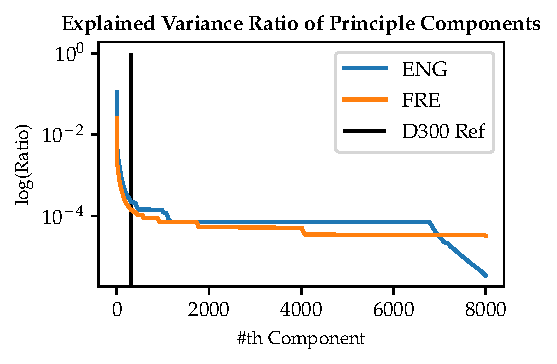
\includegraphics[scale=1]{Figures/SimDimensionSelectionVarRatio.pdf}
    \caption[Explained Variance Ratio of \code{WordNet} Embedding Principle Components]{The \code{log} of EVR of each PC in \code{WordNet} embedding space (\code{ENG}) and in WOLF embedding space (\code{FRE}). The PCs are ordered by their corresponding eigenvalues. The black vertical line is placed at the classic choice dimensionality of 300 as a reference.}
    \label{fig:SimDimensionSeletionVarRatio}
\end{figure}

\begin{figure}
    \centering
    \makebox[\linewidth]{
    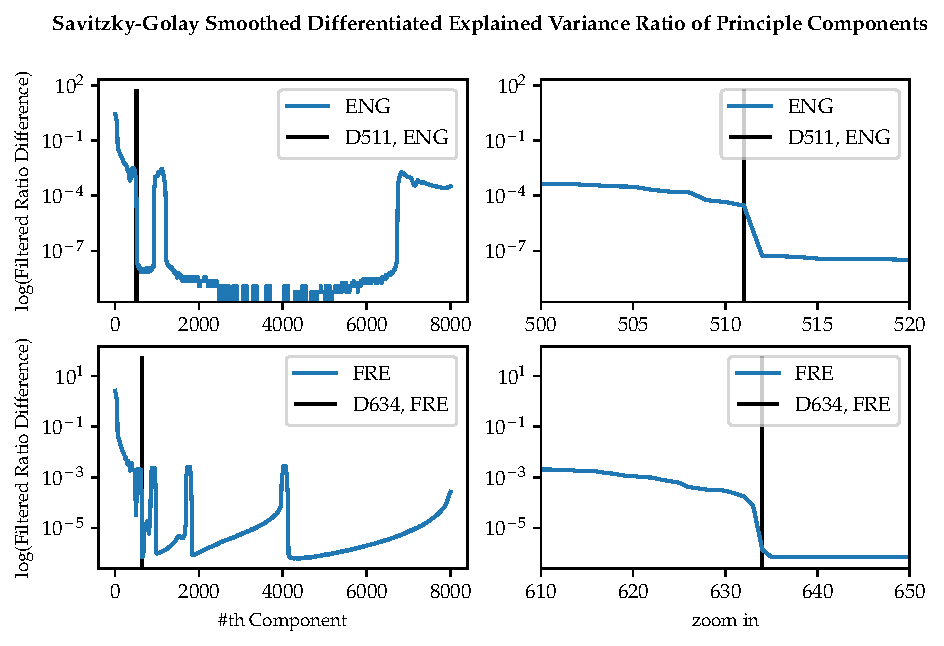
\includegraphics[width=\textwidth]{Figures/SimDimensionSelectionVarRatioDiff.pdf}
    }
    \caption[Smoothed Differentiated EVR of \code{WordNet} Embedding PCs]{\textbf{Left panels}: Savitzky-Golay filter smoothed the discrete derivative of the PC EVR signal. \code{D511} in \code{ENG} and \code{D634} in \code{FRE} are visually selected on the left border of a sufficiently wide signal valley. }
    \label{fig:SimDimensionSelectionVarRatioDiff}
\end{figure}

% code Decorrelation_French.ipynb

\subsection{Semantic Association Embedding}


\begin{equation}
    M = S.P + A 
    \label{eqn:linearmixture}
    \end{equation}

Using the linear approximation of \similarity and \association information mixture in classical SDRs (refer to Section \ref{subsection:hyplinearsemantics}), we extract \association representations from classic statistical embeddings with equation \ref{eqn:linearmixture}, where \(M\) is the mixed semantic representation space, \(S\) being the \similarity based space, \(P\) a learned projection matrix projecting the similarity space onto the mixed space, and the residual \(A\) being the \association space. The embedding spaces of interest are \(S\) and \(A\), henceforth respectively noted as \code{SIM}(short for \textbf{sim}ilarity) and \code{ASN} (\textbf{as}sociatio\textbf{n}). The two auxiliary spaces are \(P\) and \(M\), noted as \code{SIG} (\textbf{si}milarity projected on (Dep)\textbf{G}love) and \code{MIX} (\textbf{mix}ed). The projection weight \(P\) is learned via a general linear model (GLM)\footnote{\url{https://scikit-learn.org/stable/modules/linear_model.html}}, with the computational objective to minimize the L-2 norm of \(A\).

For \code{MIX} spaces, for English we use GloVe \parencite{penningtonGloveGlobalVectors2014} trained on Common Crawl with 840B tokens, 2.2M cased vocabulary and 300-dimension vectors\footnote{Pretrained data available at \url{https://nlp.stanford.edu/projects/glove/}}. For French we use DepGloVe\footnote{Pretrained data available at \url{http://alpage.inria.fr/depglove/process.pl}} \parencite{delaclergerieDepGloveSmallServer}. 

English GloVe embeddings provide word-level vectorial representations. However, since French verbs and adjectives have various inflective forms, this inflection can thin out captured semantic information if each specific form does not have sufficient frequency in a given corpus. DepGloVe aggregates semantic information by lemmatizing the tokens and attribute them with a part-of-speech (POS) tag. The main POS tags include \code{nc} (common nouns), \code{np} (proper nouns), \code{v} (verb), \code{adj} (adjectives), \code{adv} (adverbs) along with auxiliary tags.

To formulate the GLM dataset, modifications on heterogeneous embedding data are made to align the embedding spaces. Each row of the an embedding space matrix represents a lexicon unit. Since different semantic spaces have different lexicon settings, only the intersection of two vocabularies of one same language is kept in later stages. The lexicon alignment between the English embeddings is based on orthography, which is computed by string comparison. For French data, multiple text sources are converted to the same format: lemma tagged with \code{WOLF} POS tags (nouns, verbs, adjectives and adverbs). We hand coded rules to tidy up \code{WOLF} vocabulary and transformed DepGloVe's complex POS tagging entries into \code{WOLF}'s relatively simple set. Our textual data including validation task benchmarks and fMRI stimuli are also transformed to align with this strategy. Finally we manually check the vocabulary coverage against validation dataset and fMRI stimuli words, we also performed manual correction in the newly aligned space to purge algorithm erroneous results.  % code Decorrelaation_French.ipynb & Text Preprocessing.ipynb

\subsection{Embedding Validation}

Since many assumptions and approximations are made on the structure and content of semantic representation spaces, the interpretation of further results depends on the validity of the embedding construction.

The semantic ranking task depends on databases of word-pairs, each attributed with a score (usually annotated by human) which measures the proximity in terms of the semantic property defined by the task. Each semantic embedding is provided with a proximity metric, which could be derived from graph distances or vectorial distances. The score of the task is computed by calculating Pearson's and Spearman's correlation coefficient \code{r} between the embedding based word-pair proximity and the baseline. 

Conformably with other works on semantic model evaluation methods [TODO Refs, other works using the same benchmarks] \parencite{saediWordNetEmbeddings2018}, we use benchmark data provided by \textcite{rubensteinContextualCorrelatesSynonymy1965} (\textbf{RG1965}), \textcite{agirreStudySimilarityRelatedness2009} (\textbf{WS353-Similarity}) and \textcite{hillSimLex999EvaluatingSemantic2015} (\textbf{SimLex-999}) to evaluate English semantic similarity models. The only available benchmark conceived for evaluating association relations is \textbf{WS353-Association}.

\label{subsection:frenchbenchmarkdataconstruction}
\textcite{freitasSemanticRelatednessAll2016} provides translation for some of those benchmarks in French, however the provided proximity scores are heterogeneous with the original rankings. Scores for French \textbf{SimLex-99} are given by a computer semantic model, while \textbf{WS353} scores are identical with English data. The latter configuration is problematic since in different languages the translation are not exact mappings between words, and the proximities are subject to the nuanced translation choice. We manually corrected the erroneous translation of word pairs, eliminated and replaced distinct original word-pairs that are translated to the same target word-pairs, or word-pairs to the same words. Scores for the replaced word-pairs are retrieved from the English dataset. The built French benchmark data suffer from the lack of real human judgement data, thus they serve merely as indicators of semantic model performance. The modified benchmarks are made available on GitHub\footnote{commit \code{c97583f}, \url{https://github.com/nicolasying/Similarity-Association-Benchmarks}}.

\section{fMRI Voxel-Wise Encoding}


In this project and many other similar works [TODO, refs], we consider the BOLD signal of a given voxel \code{j} as a temporal signal, which is linearly composed by various independent functional sub-signals, which themselves are convolutions of separate neuron activations with a hemodynamic function: 

\begin{equation}
    \text{BOLD}_{\text{theory}, j}(t) = \sum_i {\beta_{i,j} \times f_{i}(t) * \text{hrf}(t),}
\label{eqn:boldlinear}
\end{equation}

where \(\beta_{i,j}\) is the linear coefficient of the \code{i}-th component, \(f_{i}\) is a function modeling the \code{i}-th independent functional activation, and \(\textnormal{hrf}\) is the hemodynamic function\footnote{We used packaged functions from \code{nistats, nilearn} to implement regressor construction~\parencite{abrahamMachineLearningNeuroimaging2014}.} (we use the model used in SPM at oversampling rate of 10, the hemodynamic function is illustrated in Figure \ref{fig:hrf}).

\begin{figure}
    \centering
    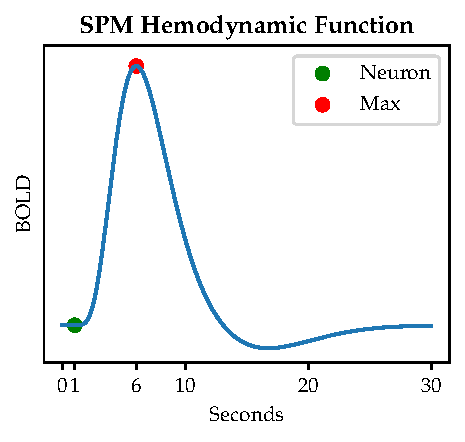
\includegraphics[scale=.8]{Figures/SPMHDF.pdf}
    \caption[SPM Hemodynamic Function]{The shape of the hemodynamic function used in the project. The modeled neural activity instantaneously fires at 1s. The maximum of the hemodynamic function is attained at 6s.}
    \label{fig:hrf}
\end{figure}


Since different voxels contain neurons of distinct (yet possibly similar) activation profiles towards stimuli, the coefficient associated with each functional component are also different for each voxel. For example, in an auditive comprehension task, the statistical distribution of GLM trained coefficients (\(\beta_{i}\) in equation \ref{eqn:boldlinear})associated to a voxel which is not implicated in audition to be near 0. Voxels containing neurons primarily associated with low-level auditive functions having non-zero \(\beta\)s for low-level auditive features.

\subsection{fMRI Textual Stimuli Preparation} 

% notebook, Text Preprocessing.ipynb
For the generation of regression features for fMRI encoding, we perform a lemmatization of the Little Prince story. First the text is parsed with syntactic dependency analysis with \code{spaCy}\footnote{version \code{2.0.16}} library and each token is attributed with a POS tag. We then used \code{FrenchLefffLemmatizer}\footnote{commit \code{ba1ef2b}. The library is publicly available on GitHub, \url{https://github.com/ClaudeCoulombe/FrenchLefffLemmatizer.}}\parencite{sagotLefffFreelyAvailable2010} library to return verbs to the infinitive form and other words to masculine singular form. POS info from \code{spaCy} helps to resolve lemmatisation ambiguity. The pipeline-generated lemma and POS tags are then manually verified and corrected\footnote{The pipeline and hand-made modifications are available at \url{https://github.com/nicolasying/Micipsa-Text-Preprocessing/blob/master/Text\%20PreProcessing.ipynb}.}.

\subsection{Regression Feature Generation}
\label{subsec:regressionfeaturegeneration}
The exact transcription of the audiobook is performed by \textcite{todorovicAnalysesIRMfLors2018}. With \code{jtrans} and \code{Praat}, the authors aligned the audio with the text by marking the onset and offset of each pronounced word in the story. To pin down the BOLD signal at a given time, we reconstruct temporal regressor functions by firstly build \(f_{i}\) in equation \ref{eqn:boldlinear}, which is essentially a sequence of bumps each occurs at the onset of a word (or content word), then we concatenate the sequence of convoluted \(D\) regressors into a design matrix of \(D\) columns.

% code TextFineTuning\LPP Onset\Lemmatisation Feature Gen.ipynb, generate_regressors.py, events2reg.py
We used four groups of features to reconstruct human listening comprehension processing cerebral activities:
\begin{enumerate}
	\item \code{RMS} (Acoustic Energy), which is the root means square of audio wave amplitude calculated on a sliding window of 10 msec, with Octave\footnote{\url{https://www.gnu.org/software/octave}}.
	\item \code{WRATE} (Word Presence), a binary temporal sequence indicating if a word is being pronounced at a given time.
	\item \code{CWRATE} (Content Word Presence), a similar binary feature to \code{WRATE}, which indicates the presence of a content word, determined by the POS tag (including nouns, verbs, adjectives and adverbs) of the lemmatised text. 
	\item \code{SIM/ASN/SIG/MIX} (Semantic Embedding-Based Features), a multi-dimensional feature set. The feature value is taken from a certain embedding defined in \(\mathbb{R}^{\vert vocabulary \vert \times n}\) space, where a particular matrix row corresponds to the content word in question. 
\end{enumerate}

\code{RMS} and \code{WRATE} are reported by post-hoc analysis of \textcite{todorovicAnalysesIRMfLors2018} as informative features. Henceforth, we define a \emph{regressor group} the regressors built from a group of features, \emph{regressor class} as the combination of regressors from the regressor group with the same name and the groups of lower feature levels. For example, the \emph{regressor class} \code{SIM} contains regressors from \emph{regressor groups} of \code{RMS}, \code{WRATE}, together with \code{SIM}.

For the ease of later design-matrix feature selection, we systematically performed orthonormalization of the convoluted feature sequences to cancel the co-linearity of the regressors. This is implemented with Gram-Schmidt process\footnote{Gram-Schmidt process is an iterative procedure applied over a set of linearly independent functions. It construct an orthogonal basis by subtracting the projection of a posteriorly positioned column over existing partial orthogonal basis (initially this basis is the first column), so that the residual of the subtracted column is linearly independent. The column residual is added to the orthogonal basis and the procedure continues until the last column is added to the basis.}~\parencite{GramSchmidtProcess2019} , where the orthogonal sequence is defined by the order of regressor classes above, and the semantic embedding based regressors inner-class order is either given by the original semantic model (\code{ASN/SIG/MIX}) or by PCA (\code{SIM}). 

\subsection{Feature Selection for Specific Corpus}
% notebook, Embedding Dimension Selection for LPP.ipynb

\code{SIM} space is constructed by taking the first PCs of a transformed ontological graph adjacency matrix, the explained variance associated to each PC is informative. As \citetitle{saint-exuperyPetitPrince1943} uses limited vocabulary, the semantic space might not be fully exploited as it was factorized with a much larger lexicon. We suspect that there might be some semantic dimensions in the semantic spaces that are not fully exhibited. It is in our interest to simplify the design matrix, leave out uninformative feature columns (those with extremely low variances) to avoid overfitting and accelerate model fitting computation. Therefore we take an investigation of the 9 design matrices (one per fMRI block) by averaging each design matrix's variance of individual regressors. After orthonormalization, the variance of regressors in higher dimension positions are of a much smaller order than the first regressors especially for PCA-factored semantic spaces. The value of threshold for column selection is determined visually to limit the number of informative regressors under 200.

\subsection{Ridge Regression with Step-wise Forward Feature Selection, Grid Search and Cross Validation}
% Ridge regression with stepwise feature selection, GridSearch Alpha 
% Github code
\label{sec:ridgemethod}
The fMRI encoding protocol is to find a function projecting our theoretical feature regressors onto BOLD amplitudes. We assume that the target BOLD value is linearly composited by individual regressors, similar in equation \ref{eqn:boldlinear}. The coefficients in the equation above is determined by the minimization of the squared difference between the predicted value given by the voxel-model and the recorded BOLD value, on a set of discrete timestamps. This is a typical regression problem tackled in Machine Learning. The computation of the coefficients is named \emph{training} or \emph{fitting} of the model. The performance of a fitted model trained on a dataset is evaluated on the accuracy of its predictions on unseen data, which indicates its \emph{generalized predictive power}.

In each fMRI recording block we have around 300 whole-brain images (refer to Section \ref{appsubsec:fmridata} for more details), totaling 2937 observations. Researchers \parencite{huaOptimalNumberFeatures2005} found that in GLM the optimal number of uncorrelated informative features is \(N - 1\) where \(N\) is the number of observation, and \(\sqrt{N}\) if features are correlated. Although we have numerically de-correlated the regressors, we nevertheless cannot assume the conceptual independency. Thus 200 regressors might outnumber the recommended feature size. To avoid potential overfitting of regression models, we use Ridge regression to penalize the attribution of large coefficients. Equation \ref{eqn:ridge} is the minimization problem posed by Ridge regression, with \code{j} fixed for voxel \code{j} and \(N_j\) the number of features used by voxel \code{j}. Strong penalization reduces potential noises by limiting the chance of particular feature columns weighing too much on final prediction, therefore promotes the robustness and generalizability of a fitted model.

\begin{equation}
    \min_{\beta_{i,j}}{\sum_{t}{\vert\sum_{i}^{N_j}{\beta_{i,j} \times f_{i}(t) * \text{hrf}(t)} - \text{BOLD}_{\text{real}, j}(t)\vert ^2} + \alpha_j \sum_{i}^{N_j}{\beta_{i,j}^2}}
\label{eqn:ridge}
    \end{equation}

Ridge regression fitting algorithm requires a hyper-parameter (\(\alpha\)) to adjust the severity of large-coefficient penalty. There's no empirically predetermined optimal choice of the value for similar project settings, thus we test a range of candidates by fitting different models and evaluate their performance. 

We also assumed the heterogeneity of voxel activation profile towards different functional features. In order to maximize the predictive power of models, we trial multiple combinations of feature columns on each voxel-model. Limited by the computation time, we do not test all the combinations of individual features which could results in an exponential complexity, but use \emph{step-wise forward} feature selection by the order of feature classes (Section \ref{subsec:regressionfeaturegeneration}). 

A major difference of this project from \textcite{todorovicAnalysesIRMfLors2018, verdierEncodageActiviteNeuronale2018} is the voxel-specific configuration. Our pilot regression experiments partially replicated the original experience \parencite{todorovicAnalysesIRMfLors2018} on French data. The results showed that fixing one regularization parameter for all models (including non-semantic models and \code{MIX} models) cannot fully exploit the power of the supplied regressors. The fixed \(\alpha\) preferentially improves the regression performance for certain models. 

By prior experiences, a search range for \(\alpha\) is fixed beforehand. We sampled 34 \(\alpha\)s from the defined range and up to 32 feature dimension candidates, in hope of including the near-optimal hyper-parameter combination for the regression of each voxel-level model. The list of tested parameters are fixed in each model's config file\footnote{For example, \code{ASN} is configured as \url{https://github.com/nicolasying/Micipsa/blob/master/models/fr/rms-wrate-cwrate-asn200/config.json}. Please refer to Section \ref{appsubsec:regressionparameters} for tested \(\alpha\) value, feature selections.}.

In our project, for each voxel of a subject and each combination of \(\alpha\) value candidate and feature selection, we adopt the common practice of Cross Validation (CV), where we generate 9 different regression models by training on 8 runs of fMRI recording leaving one out for validation, and test their performance on the left run by computing the coefficient of determination (\code{r2}) by comparing model predicted BOLD values and real observations. We will henceforth name the model validated on fMRI block \code{i} \emph{run} \code{i}. \code{r2} measures the proportion of the variance in the BOLD signal that is predictable from the feature regressor data. An \code{r2} of 1 indicates that the regression predictions perfectly fit the data.

We normalized all feature regressors and voxel-wise fMRI signal sequences for the facility of inter-individual comparison and group-level analysis. To reduce the total computation time, we filtered out unimportant voxels in the images by computing a multi-EPI mask.\footnote{The \code{nilearn.masking.compute\_multi\_epi\_mask} uses the mask-finding algorithms to extract masks for each session of subject, and then keeps only the main connected component of a given fraction  of the intersection of all the masks.}

\section{Analysis}

The Ridge regression pipeline results to \[ \lvert \text{Subject} \rvert \times \lvert \text{Voxels} \rvert \times \lvert \alpha~\text{candidates} \rvert \times \lvert \text{feature selection} \rvert \times \lvert \text{CV} \rvert \] fitted voxel-models for each semantic space. 


\subsection{Incremental Nested Model Sequence}

First we investigate the validity of regression results. 

For each individual voxel in 9 cross-validation sessions, \( \lvert \alpha~\text{candidates} \rvert \times \lvert \text{feature selection} \rvert \) results are given. For each cross-validated model, we select the highest \code{r2} among \(\alpha\)s and feature selections within feature classes. For example, for voxel \code{j} \code{CWRATE} feature class result, we take the maximal \code{r2} score for each voxel \code{j} model among all the scores found with \code{RMS}, \code{RMS+WRATE} and \code{RMS+WRATE+CWRATE} features and all tested \(\alpha\)s. This selection reduces the number of reported scores to \( \lvert \text{Subject} \rvert \times \lvert \text{Voxels} \rvert \times \lvert \text{feature classes} \rvert \times \lvert \text{CV} \rvert \). This reporting approach is proposed due to the overfitting problem of regression models: the addition of extra features does not necessarily translate into a higher performance. If a model overfits (i.e. \code{r2} declines) with the addition of features, the overfitted nesting-model results are substituted with un-overfitted nested-model ones so that on whole-brain maps the best voxel-models are always visualized. For example, if a voxel's \code{r2} performances with different regressor classes are ranked as follows: \code{CWRATE} > \code{SIM} > \code{RMS} = \code{WRATE}, then in whole-brain visualization and model comparative analyses, \code{WRATE} \code{r2} is used for \code{RMS} and \code{WRATE}, and \code{CWRATE} \code{r2} for both \code{CWRATE} and \code{SIM}. Thus the contrast of \code{SIM} against \code{CWRATE} is zero rather than a negative number.

For each feature class, the subject-wise result whole-brain map and the group-wise map are visualized by averaging across \(\lvert \text{CV} \rvert \) and \( \lvert \text{Subject} \rvert \times \lvert \text{CV} \rvert \) voxel- and feature-class-specific results. With each additional feature class starting from \code{WRATE}, the improvement of \code{r2} scores are also plotted. With the downward-inclusive best model selection, only non-negative contrasts are reported. 
 
\begin{equation}
    \begin{split}
    \text{F} &= \frac{\frac{\code{RSS}_{\text{restricted}}-\code{RSS}_{\text{full}}}{p_{\text{full}}-p_{\text{restricted}}}}{\frac{\code{RSS}_{\text{full}}}{n-p_{\text{full}}}}, \\
    &\text{where } p\text{ is number of features, }n\text{ is number of samples.}
    \end{split}
\label{eqn:waldF}
    \end{equation}

The statistical significance of improvement is computed by Wald F-test (Equation \ref{eqn:waldF} on model validation scores. The Wald F-test compares the residual sum of squares (\code{RSS}) of a restricted model and a full model nesting the former one, with the null hypothesis suggesting that the full model does not provide a significantly better data fit than the restricted one. The Wald test penalizes large feature set, and takes the number of observations into account, thus is more restrict than tests comparing \code{r2} scores. The \code{RSS} is computed from \code{r2} given that the data are centered and normalized (Equation \ref{eqn:rssr2} for voxel \code{j}).


\begin{equation}
    \begin{split}
         \code{RSS}_j &= \sum_{t=0}^{n} {(\text{BOLD}_{\text{real}, j}(t) - \text{BOLD}_{\text{predict}, j}(t))^2} \\
         \code{r2}_j &= 1 - \frac{\sum_{t=0}^{n}{(\text{BOLD}_{\text{real}, j}(t) - \text{BOLD}_{\text{predict}, j}(t))^2}}{\sum_{t=0}^{n}{(\text{BOLD}_{\text{real}, j}(t) - \text{BOLD}_{\text{average}, j})^2}} \\
         &= 1 - \sum_{t=0}^{n}{(\text{BOLD}_{\text{real}, j}(t) - \text{BOLD}_{\text{predict}, j}(t))^2} \\
         &= 1- \code{RSS}_j
        \end{split}
\label{eqn:rssr2}
    \end{equation}

For each addition of \emph{feature group}, we perform a Wald F-test within each cross-validation session for each voxel. The full and restricted model scores are selected among \( \lvert \alpha \text{ candidates} \rvert \times \lvert \text{feature selection} \rvert \) within the corresponding \emph{feature class}. The number of features of each model are determined by feature selection, and the number of samples is the fMRI image number of the cross-validation session.

At individual analysis level, for each contrast of each individual voxel, \( \lvert CV \rvert \) F-tests are computed. For the final significance visualization, we compute the geometric mean of p-values over \(\lvert CV \rvert \) runs. We then plotted the statistical map by thresholding the p-value by uncorrected 0.05, uncorrected 0.001 and Bonferroni multi-comparison corrected 0.05. For group analysis, the geometric mean is computed over \(\lvert subject \rvert \times \lvert CV \rvert \) observations. 

To pin down cortical regions well modeled by a particular class of model, we select the best 0.1\% and 1\% voxels and report voxel-clusters larger than 1500 \(\text{mm}^3\) (47 voxels). For \code{r2} difference maps, smaller regions are permitted (500 \(\text{mm}^3\) (16 voxels)), the lower bound of voxel-wise Wilcoxon statistic significance of the clusters are also reported. With F-test results, we report voxels surviving three-levels of significance thresholds.

Without prior hypothesis on semantic embeddings, the regression pipeline is expected to recover at least auditive cortical areas for \code{RMS} feature regression by plotting the whole-brain map of \code{r2}. The additional features' and contrast maps' validity are backed by the validity of \code{RMS} activation regularities.

\subsection{Embedding Contrasts}
The key comparison of regression results is the contrast between \code{SIM} and \code{ASN} semantic models. The comparison computational procedure is inspired by the non-nested model comparison pipeline \parencite{merkleTestingNonnestedStructural2016}. Our method is divided into two steps: first we verify the structural difference between the design matrices given by each model, secondly we compare the model's regression results if the design matrices are found nonequivalent. The pipeline is detailed in Section \ref{appsubsec:nonnestedcompmeth}.

For voxel-model regression result contrasts, the \code{r2}s follow distributions described by \(F(k-1, n-k)\), where \(k\) is the number of features and \(n\) is the number of observation. Since across semantic models, the feature dimensions are heterogeneous, \code{r2} scores have distinct score distributions. Therefore we adopted the nonparametric Wilcoxon signed-rank test to test the significance of \code{r2}-differences between semantic models. 

For voxel-level group contrasts, we take two paired groups of \code{r2} scores, each composed by \( \lvert \text{Subject} \rvert \times \lvert \text{CV} \rvert \) observations. The Wilcoxon test yields a W statistic and a p-value for each voxel. For individual contrasts, since \(\lvert \text{CV} \rvert < 20\), the Wilcoxon test is tested with T statistic. For a group size of 9 observations, T critical values for two-tailed alternative hypothesis are 8, 5, 3, 1 for alpha (statistic power) < 0.1, 0.05, 0.02, 0.01.

In result

\subsection{ROI-level Analysis}

With Region-of-Interest (ROI) analysis, we aim to filter out inter-subject variances and find relatively stable loci of each semantic network. We replicated \textcite{pattersonWhereYouKnow2007}'s peak selection method to select the reported peaks in temporal region from the relevant literatures reporting the activation peaks of semantic tasks~\parencite{devlinSusceptibilityInducedLossSignal2000, mummerycatherinej.GeneratingTigerAnimal1996, priceMetaanalysesObjectNaming2005, rogersAnteriorTemporalCortex2006, brightUnitaryVsMultiple2004, crinionTemporalLobeRegions2003, scottIdentificationPathwayIntelligible2000, gorno-tempiniIdentificationFamousFaces2001, nakamuraFunctionalDelineationHuman2000, gorno-tempiniNeuralSystemsSustaining1998, tsukiuraDissociableRolesBilateral2006, nakamuraNeuralSubstratesRecognition2001, binderHumanTemporalLobe2000,davisHierarchicalProcessingSpoken2003, scottNeuralCorrelatesIntelligibility2006, ferstlEmotionalTemporalAspects2005, noppeneyRetrievalVisualAuditory2002, papathanassiouCommonLanguageNetwork2000, tranelNamingSameEntities2005, mummeryDualProcessModelSemantic1999, smallRoleRightAnterior1997, simonsNeuralMechanismsVisual2003, vuilleumierMultipleLevelsVisual2002, grossmanNeuralBasisSemantic2003},
% code ROI\Tal2MNI_ROI_gen.ipynb
and obtained the list of ROI by constructing a 7-mm diameter sphere around the peaks.

We completed the ROI list by intersecting the original ROI mask with gray-matter mask, and added classic language-related brain anatomical areas including Superior Temporal Gyrus (STG), Inferior Frontal Gyrus (IFG), IFG pars opercularis (IFGoper), IFG pars orbitalis, IFG pars triangularis, Temporal Lobe (TL), Temporal Pole (TP), posterior Superior Temporal Sulcus, Temporoparietal Junction (TPJ), anterior TL, Putamen, Middle TG, left Premotor Cortex,\parencite{pallierCorticalRepresentationConstituent2011}. The ROI centroids are reported in Section \ref{appsubsc:roilist}.

\subsubsection{ROI Statistical Test}
We computed the ROI-average \code{r2}, and used the same Wilcoxon signed-rank test as voxel-wise analysis.
\chapter{Results} % Main chapter title

\label{chap:results} % For referencing the chapter elsewhere, use \ref{Chapter1} 

\section{Semantic Embeddings}
\subsection{Validation on English Data}
For \code{SIM} space, we used the English \code{WordNetEmbedding} trained on the first 15,000 frequent words and benchmark dataset vocabulary. We kept 511 first PCs by following the method in section \ref{subsec:semanticsimilaritymethod}.

The intersection of \code{SIM} space and the Common Crawl vocabulary used in \code{MIX} space resulted to 8157 words. 

The linear regression model mapping \code{SIM} to \code{MIX} produced a \code{r2} score of 0.1662.

Figure \ref{fig:EngDecorVarRatio} shows the PCA analysis of the resulting 4 semantic spaces. Table \ref{tab:engdecorrelationscores} shows the semantic ranking task results: though we have not completely dissociated each resulting semantic space with irrelevant semantic axis, a clear dominance of \association semantic signal is present in \code{ASN} space. 

\begin{table}
\centering
\begin{ThreePartTable}
    
\begin{tabularx}{\textwidth}{RRRRll}
    \multicolumn{6}{l}{\tabhead{English Semantic Space Semantic Ranking Task Results}} \\
\toprule
\tabhead{Semantic Space} & \tabhead{Vocabulary Size} & \tabhead{Dimension} & r & \tabhead{SimLex-999} & \tabhead{WS353-ASN} \\  
\midrule
\mr{2}{*}{\code{SIM}} & \mr{2}{*}{15K} & \mr{2}{*}{511} & Pearson & 0.5060 & \textbf{0.0279}\tnote{1} \\  
&  &  & Spearman & 0.4989 & \textbf{0.0193}\tnote{2}   \\  
\midrule
\mr{2}{*}{\code{MIX}} & \mr{2}{*}{2.2M} & \mr{2}{*}{300} & Pearson & 0.3946 & 0.6091 \\  
&  &  & Spearman & 0.3752 & 0.5709 \\  
\midrule
\mr{2}{*}{\code{ASN}} & \mr{4}{*}{8157} & \mr{4}{*}{300} & Pearson & 0.1953 & 0.5633 \\  
&  &  & Spearman & 0.2133 & 0.5918 \\ 

\cmidrule{1-1} \cmidrule{4-6}
\mr{2}{*}{\code{SIG}} &  &  & Pearson & 0.4929 & 0.2091 \\  
&  &  & Spearman & 0.4994 & 0.1678 \\  

\cmidrule{2-6}
\multicolumn{4}{r}{Out of Vocabulary} & 0.002 & 0.024 \\  
\midrule \midrule
\mr{2}{*}{Baseline\tnote{3}} & \mr{2}{*}{13k} & \mr{2}{*}{850} & Pearson & 0.50 & 0.32 \\  
    &  &  & Spearman & 0.52 & 0.33 \\  
\bottomrule
\end{tabularx}
\begin{tablenotes}
    \footnotesize
    \item[1] p-value=0.6626
    \item[2] p-value=0.7629
    \item[3] Baseline is reported by \cite{saediWordNetEmbeddings2018}. The 13k words are selected cue words in psycholinguistic experiments. They show the best performance among all tested models.
\end{tablenotes}
\end{ThreePartTable}
\caption[English Semantic Space Semantic Ranking Task Results]{\code{SIM} achieves almost the same performance as the baseline in \similarity benchmark, while it cancels out the 
\association score. \code{MIX} space performs well in both task-sets, with a slight preference for \association, consistent with \parencite{lapesaContrastingSyntagmaticParadigmatic2014}'s conclusion. \code{ASN} has comparable scores in \association with \code{MIX}, but still have a non-zero score in \similarity. Such is also the case for \code{SIG} compared with \code{SIM}.\label{tab:engdecorrelationscores}}
\end{table}

\begin{figure}
    \centering
    \makebox[\linewidth]{
    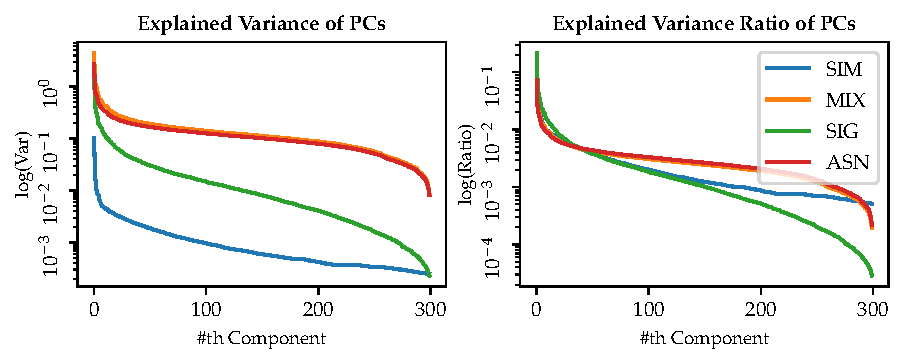
\includegraphics[scale=1]{Figures/EngDecorVarRatio.pdf}
    }
    \caption[EVR of 4 Semantic Spaces]{PCA of 4 semantic spaces of 8157 vocabulary. \textbf{Left panel}: While the variance of \code{SIM} is systematically lower than other three spaces, its projection (\code{SIG}) has larger variances. The suppression of \code{SIG} from \code{MIX} has little impact on the model's variance. \textbf{Right panel}: \code{SIG} and \code{SIM} have a denser variance concentrated on first PCs, while \code{ASN} and \code{MIX} have more homogeneous variance distributions.} 
    \label{fig:EngDecorVarRatio}
\end{figure}

\subsection{Application on French data}

Provided with the methodological success of English data, we applied the same algorithm against French data.

For \code{SIM} space, we used the French \code{WOLFEmbedding} with POS tag trained on all the available vocabulary. We kept 634 first PCs.

After rule-based and manual matching, the intersection of \code{SIM} space and the \code{MIX} space vocabulary resulted to 24519 distinct lemma with POS tags.

The linear regression model mapping \code{SIM} to \code{MIX} produced a \code{r2} score of 0.0776, which is lower than the English score, indicating a smaller informational overlap between the two embedding models.

Figure \ref{fig:FreDecorVarRatio} shows a similar PCA analysis. Though indicative, we tested the resulting semantic spaces using the same tasks against our indicative gold-standard data (section \ref{subsection:frenchbenchmarkdataconstruction}). The results (table \ref{tab:fredecorrelationscores}) puts the validity of \code{ASN} space into question: it seems to contain both \similarity and \association information.

\begin{figure}
    \centering
    \makebox[\linewidth]{
    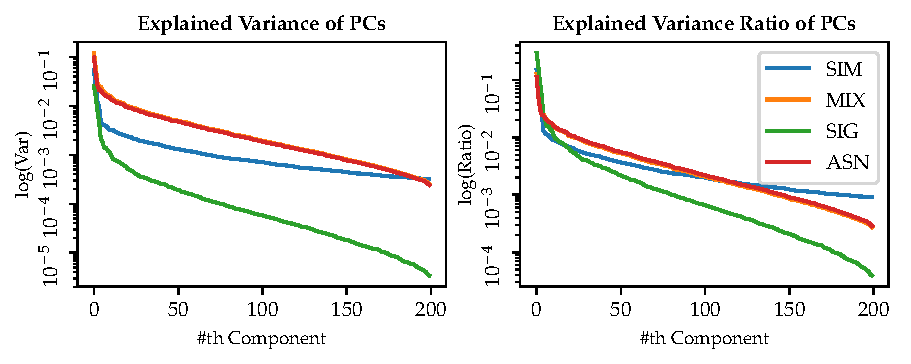
\includegraphics[scale=1]{Figures/FreDecorVarRatio.pdf}
    }
    \caption[EVR of 4 French Semantic Spaces]{PCA of 4 semantic spaces of 24519 vocabulary. \textbf{Left panel}: Due to the poor linear correlation found between \code{SIM} and \code{MIX}, the variance of \code{SIG} is systematically lower than the other three spaces, its projection (\code{SIG}) has larger variances. The suppression of \code{SIG} from \code{MIX} has also little impact on the model's variance. \textbf{Right panel}: \code{SIG} has a denser variance concentrated on first PCs, while the other three spaces have more homogeneous variance distributions.\label{fig:FreDecorVarRatio}} 
    
\end{figure}

\begin{table}
    \centering
    \begin{ThreePartTable}
    
    \begin{tabularx}{\textwidth}{RRRRll}
        \multicolumn{6}{l}{\tabhead{French Semantic Space Semantic Ranking Task Results}} \\
    \toprule
    \tabhead{Semantic Space} & \tabhead{Vocabulary Size} & \tabhead{Dimension} & r & \tabhead{SimLex-999} & \tabhead{WS353-ASN} \\  
    \midrule
    
    \mr{5}{*}{SIM} & \mr{4}{*}{56665} & \mr{4}{*}{634} & Pearson & 0.3291 & \textbf{0.1039} \\  
    &  &  & p-value & 0 & 0.1061 \\  
    \cmidrule{4-6}
    &  &  & Spearman & 0.2812 & \textbf{0.0511} \\  
    &  &  & p-value & 0 & 0.4273 \\  
    \cmidrule{2-6}

    \multicolumn{4}{r}{Out of Vocabulary} & 0.048 & 0.04 \\  
   \midrule

   \mr{4}{*}{MIX} & \mr{14}{*}{24519} & \mr{14}{*}{200} & Pearson & 0.0940 & 0.1520 \\  
   &  &  & p-value & 0.0047 & 0.0197 \\  
   \cmidrule{4-6}

    &  &  & Spearman & 0.1449 & 0.2078 \\ 
    &  &  & p-value & 0 & 0.0014 \\  

    \cmidrule{1-1} \cmidrule{4-6}

   \mr{4}{*}{ASN} &  &  & Pearson & \textbf{0.0629} & \textbf{0.1116} \\  
   &  &  & p-value & 0.0590 & 0.0879 \\  
   \cmidrule{4-6} 
    &  &  & Spearman & 0.0771 & 0.1566 \\  
    &  &  & p-value & 0.0206 & 0.0162 \\  

\cmidrule{1-1} \cmidrule{4-6}

   \mr{4}{*}{SIG} &  &  & Pearson & 0.2541 & \textbf{-0.0044} \\  
   &  &  & p-value & 0 & 0.9458 \\  
   \cmidrule{4-6}

    &  &  & Spearman & 0.3121 & \textbf{-0.0078} \\  
   &  &  & p-value & 0 & 0.9050 \\  

    \cmidrule{2-6}

    \multicolumn{4}{r}{Out of Vocabulary} & 0.0797 & 0.0711 \\  

    \bottomrule
    \end{tabularx}
    \begin{tablenotes}
        \footnotesize
        \item Scores marked in bold have a p-value larger than 0.05.
    \end{tablenotes}
    \end{ThreePartTable}
    
    \caption[French Semantic Space Semantic Ranking Task Results]{The results are consistent with English semantic spaces, despite the poor quality of French benchmark datasets. \code{SIM} has high performance in \similarity and negligible \association scores. The relatively poor de-correlation between \code{SIM} and \code{MIX} resulted a \code{ASN} still containing abundant \similarity information. \code{SIG} however, cancels out completely \association information even compared with \code{SIM} while retained \similarity signals.}
    \label{tab:fredecorrelationscores}
    \end{table}

We visualized the French semantic spaces with an embedding projector\footnote{Published as a TensorFlow component, available at \url{https://projector.tensorflow.org/}. The entries in the embedding space is presented by a sphere positioned in a 3D space, of which the coordinates are by default calculated with the first 3 PCs.} to visually control embedding quality via several exemplar lexicons and its vectorial neighbors. Based on this analysis (more details in section \ref{appsubsec:projectorvisu}), we are convinced that French \code{ASN} has a predominant \association preference.

\section{Computational Analysis of Ridge Regression}

\subsection{Regressor Generation}

\subsubsection{Vocabulary Coverage}
Each word (lexicon, lemma) in the narrated story used in fMRI experience is associated with its \code{RMS} acoustic feature temporal evolution and its semantic values in different spaces. However some of the words are not all available in our obtained spaces (table \ref{tab:lppcoverage} and \ref{apptab:lppcoverage}). When generating regressors, the semantic vectors are set to zero for out-of-vocabulary lemmas. 

\begin{table}
    \centering
    \begin{ThreePartTable}  
    \begin{tabularx}{\textwidth}{L *{10}{R}}
    \multicolumn{11}{l}{\tabhead{The Little Prince Vocabulary Coverage}} \\
    \toprule
    &  & \multicolumn{9}{l}{\tabhead{\# Instances in fMRI Recording Session}} \\
    \toprule
    \mr{2}{*}{Story} & \textbf{T} & 725 & 812 & 860 & 762 & 732 & 902 & 819 & 712 & 802 \\
    & \textbf{V} & F & 812 & 860 & 762 & 732 & 902 & 819 & 712 & 802 \\
    \midrule
    \mr{4}{*}{\parbox{0.8cm}{\code{SIM} 56665}} & TM & 36 & 30 & 32 & 27 & 30 & 33 & 24 & 30 & 27 \\
    & \% & F & 812 & 860 & 762 & 732 & 902 & 819 & 712 & 802 \\
    & VM & F & 812 & 860 & 762 & 732 & 902 & 819 & 712 & 802 \\
    & \% & F & 812 & 860 & 762 & 732 & 902 & 819 & 712 & 802 \\
    \midrule
    \mr{4}{*}{\parbox{0.8cm}{\code{ASN} /\code{MIX} /\code{SIG} 24519}} & TM & 48 & 47 & 38 & 37 & 48 & 60 & 35  & 37 & 41 \\
    & \% & F & 812 & 860 & 762 & 732 & 902 & 819 & 712 & 802 \\
    & VM & F & 812 & 860 & 762 & 732 & 902 & 819 & 712 & 802 \\
    & \% & F & 812 & 860 & 762 & 732 & 902 & 819 & 712 & 802 \\
    \bottomrule
    \end{tabularx}
    \end{ThreePartTable}
    \caption[The Little Prince Vocabulary Coverage in Semantic Spaces]{\textbf{T}: Token, \textbf{V}: Vocabulary, M: Miss\label{tab:lppcoverage}}
    \end{table}



\subsubsection{Corpus-Targeted Semantic Feature Selection}

The PCA dimension cutting methods presented in section \ref{subsec:semanticsimilaritymethod} produced 634 feature dimensions for French \code{SIM}. \code{ASN}, \code{MIX} and \code{SIG} have the same dimensionality as the original DepGloVe space. 

After have generated regressors with word onset timestamps and semantic representation vectors, the variance of resulting regressors are computed and visualized in figure \ref{fig:freSIMRegVar}, \ref{fig:freASNRegVar}, \ref{fig:freSIGRegVar} and \ref{fig:freMIXRegVar}. We selected the threshold of \(10^{-8}\), which resulted 100 informative regressors for \code{SIM} space [TODO, list of regressors in SI], and all 200 regressors generated by each of other three spaces survived the selection. 

\begin{figure}
    \centering
    \makebox[\linewidth]{
    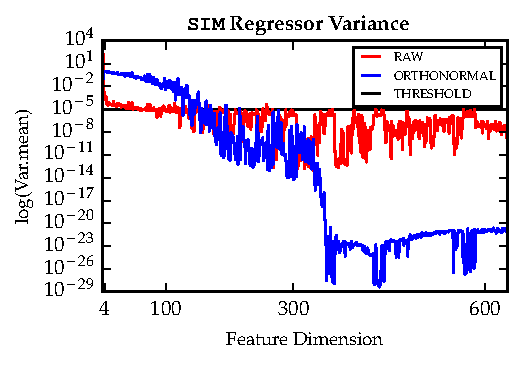
\includegraphics[scale=1]{Figures/SimDimensionSelectionRegLPP.pdf}
    }
    \caption[French \code{SIM} Regressor Variances]{Statistics on semantic regressors of 9 fMRI runs. \code{RAW} stands for regressor values directly after hemodynamic convolution, \code{ORTHONORMAL} stands for de-linearized regressors after Gram-Schmidt process. \code{THRESHOLD} is fixed at \(10^{-8}\). \textbf{Upper panel}: The minimal variance among 9 runs are shown. As \code{SIM} has a high concentration of explained variance in the first PCs (figure \ref{fig:FreDecorVarRatio}), the \code{RAW} regressors decline correspondingly for low-rank PCs. \code{ORTHONORMAL} regressors suffer more significantly and retained almost no information for the second half PCs. \textbf{Lower panel}: The average value of regressors across 9 runs shows a similar trend as the analysis on min values.} 
    \label{fig:freSIMRegVar}
\end{figure}

\begin{figure}
    \centering
    \makebox[\linewidth]{
    \includegraphics[scale=1]{Figures/ASNDimensionSelectionRegLPP.pdf}
    }
    \caption[French \code{ASN} Regressor Variances]{\code{THRESHOLD} is fixed at \(10^{-8}\). The non-PCA-transformed \code{ASN} space produced relatively more informative regressors.[TODO, figure xlabel, replace Component by dimension]} 
    \label{fig:freASNRegVar}
\end{figure}





\subsection{Impact of \(\alpha\) and Effective Feature Dimensionality}
For each of four semantic models, we generated design matrices for each fMRI session with 103 and 203 features. We sampled [TODO] \(\alpha\) and up to[TODO] feature dimension candidates by past experience, in hope of including the near-optimal hyper-parameter combination for the regression of each voxel-level model. The list of tested parameters are fixed in each model's config file\footnote{For example, \code{ASN} is configured as \url{https://github.com/nicolasying/Micipsa/blob/master/models/fr/rms-wrate-cwrate-asn200/config.json}.}, and a typical example is available in section \ref{appsubsec:alphadim}.

We selected four typical voxels in post-hoc from the regression results of run [TODO] of subject [TODO]. Each voxel is the best modeled voxel who maximizes \code{r2} among all \(\alpha\)s using only partial feature information of a certain regressor class. For example, a \code{CWRATE} class typical voxel is a voxel of which the best \code{r2} is achieved with \emph{all} first 3 features (\code{dim=3}). 

[TODO: figure Surface plot of dim/alpha]

The optimal \code{r2}s of typical voxels are never attained at the upper bound of \(\alpha\) and dimension space [TODO, refer to precedent figure]. We plotted the head-map for all voxels from session [TODO] of subject [TODO] to verify if it is also the case at the whole-brain level. In figure [TODO], each cell represents an \(\alpha\) and dimension combination. The color indicates the number of voxels having its global optimality with a given parameter set. [Todo: heat-map of dim/alpha] Since we do not have a growing trend of voxel population, this hypothesis that our parameter combination contains the near-optimal configuration for each voxel is accepted.

\section{Cognitive Analysis of fMRI Encoding}
\subsection{Basic Models}
Figure [TODO ind and group] are the whole-brain plot for regression analysis. Not that if a model overfits (i.e. \code{r2} declines) with the addition of features, the overfitted results are substituted with un-overfitted ones. Therefore, figure [TODO hist] plots the distribution of voxel-wise optimal \code{r2} (of run[], subject [] for exemplar illustration) and tracks the effective improvement when adding further feature spaces, unaffected by the overfitting problem. 

If we consider the regression model performance at each voxel as a neural activation against a potential modeled guess of local BOLD activity,
then \code{r2} activation of each individual is most of the time temporal and sometimes frontal, less often parietal even occipital. The activation peaks are found at [TODO, report peaks in table] mostly in bilateral mSTS/pSTS [TODO, ROI analysis] for all \code{RMS}, \code{RMS+WRATE} and \code{RMS+WRATE+CWRATE} models. 

With the presence of \code{RMS}, \code{WRATE} adds marginal information [TODO: Orhtonormal data on RIF]. However, \code{CWRATE} always brings significant improvements. The maximal improvement over \code{r2} by the single feature often exceeds a half of the best \code{r2} of the restricted model for precedently poorly modeled voxels. [TODO, histogram \& superposition of images]
This might be a direct implication of orthonormalization of our feature regressors.

The inter-subject variability is particularly pronounced. On averaging the \code{r2} of all 20 subjects, we are able to recover peak areas in bilateral mSTG/pSTS [TO verify]. The averaged improvement of \code{CWRATE} is located at TP, ITG, occipital and IFG[TODO verify]. 

\subsection{\emph{Similarity} Nested Model}

With \similarity semantic models, the constructed \code{SIM} features bring similarly significant improvements as \code{CWRATE}. The improvement found by \code{SIM} addition is more regular: clustered voxels in bilateral aSTS mSTS mITS, s parietotemporal, and IFG [TODO, check name]. Individuals show a lateralization preference for left hemisphere. 

[TODO, ind and group maps: r2 base, r2 full, r2 diff, F test(for ind)]


\subsubsection{First Observations on Semantic Hub}

[TODO, ROI analysis: F-test ROI, count]

\subsection{\emph{Association} Nested Model}
The addition of \code{ASN} features resulted more powerful results [TODO: powerful?] than \code{SIM}. Each voxel cluster found with \code{ASN} tends to be more extensive, [report significance regions]. [TODO, inferior parietal ]

\subsection{\emph{Similarity}/\emph{Association} Contrast}

\subsection{Full Embedding}
% \section{Behavioral Control} 
\chapter{Discussion} % Main chapter title

\label{chap:discussions} 

%----------------------------------------------------------------------------------------
\section{Back to Hypothesis}

Our hypothesis argues for a \similarity based semantic hub internal organization and \association for that of other non-hub components. By modeling \similarity processing axis by \code{SIM}\slash \code{SIG} and \association by \code{ASN} features, the \code{SIM}\slash \code{SIG}-\code{ASN} voxel-performance contrast should align with the semantic hub versus non-hub spatial map, namely a bilateral (ventrolateral) aTL centered contrast. 

By indicating the presence of a content word, thus the necessity of semantic processing, the regression model improved the voxel-models located in bilateral mid temporal pole (TP), posteroinferior temporal gyrus (pITG) including left middle fusiform gyrus (mFG) and frontopolar prefrontal cortex (fpPFC). This finding is compatible with the hypothesis as both \similarity and \association regions are revealed.

The constructed \code{SIM} features most improved voxels located in bilateral middle temporal gyrus (MTG) and left superior parietal lobule and right angular cortex, \code{SIG} in posterior inferior TG, right angular gyrus (AG) and bilateral inferior frontal gyrus pars triangularis (IFGtri). \code{ASN} improvements report voxel clusters implicated in left superolateral FG, bilateral IFGtri, left medial superior frontal gyrus, left middle cingulate cortex, pSTS and other visual areas. The \code{SIM}-\code{ASN} contrast revealed preferential models for \code{SIM} in left superior frontal cortex (SFC) and anterior cingulate cortex (ACC), and before correction bilateral pSTG, left aMTG, right mMTG. The \code{SIG}-\code{ASN} contrast found \code{SIG}'s advantage in primary auditory cortex, posterior fusiform gyrus. 

Our findings for \code{SIM}/\code{SIG} modeling \similarity are not convergent on temporal organizational properties. None of ventroanterior aspect of the TL is found by any of the contrast. No prior evidences suggest SFC and ACC's implication in pure \similarity processing.  

Nevertheless, pure \association areas are confirmed to be principally located in occipital area including middle and inferior aspects of occipital cortex. Bilateral BA17/18 in calcarine, cuneus, BA19, lingual gyrus are only found related with \code{ASN}.

Before examining the validity of our hypothesis, several potential confounds impact the power of this study.

\section{Precise and Informative Semantic Feature Design}

\subsubsection{Impact of \code{CWRATE}}

\code{CWRATE} indicates the necessity of semantic retrieval and processing when a stimuli is presented. Both \similarity and \association aspects are wrapped in the feature. Most of the voxel-clusters improved by \code{CWRATE} are associated with visual recognition\slash identification (posterior fusiform), visual association (BA18/19, V2,3,4,5), premotor (rolandic oper BA6) visuo-motor coordination (Precuneus, Superior Occipital). But two aTL regions in MTP are also reported, which are near by the neural fiber convergence zone. 

As \code{CWRATE} is a shared feature for \code{SIM}\slash\code{SIG} and \code{ASN} models, orthonormalizing embedding feature regressors against \code{CWRATE} suppresses a large proportion of semantic-axis-specific signal in fMRI encoding, potentially weakening the contrast between \code{SIM} and \code{ASN}.

\subsubsection{Better Constructions of \code{SIM}}

\code{SIM} models have lower regression scores than \code{ASN}, this could be caused by a limited extent of \similarity processing neurons compared to \association, or the lack of quality control of the \code{SIM} embedding. The English \code{SIM} embedding is well constructed: \code{WordNet} is widely used, the resulting embedding's quality is assured by semantic evaluation tasks. Whereas for French the ontology is built upon the algorithm-generated \code{WOLF}, which makes use of multilingual resources and is composed of translation-based synsets. Additionally, the French semantic evaluation task datasets are not tested. There are potentially more appropriate construction of a valid \similarity embedding.

From a pure computational aspect of view, \textcite{bullinariaExtractingSemanticRepresentations2012} found that removing the initial PCs of singular-value-decomposed (SVD) semantic matrices improves the performance on multiple semantic tasks (such as TOEFL, Distance Comparison, Semantic Categorization and Clustering Purity, fMRI encoding/decoding tasks are not included). In our project we did not remove the initial PCs nor did \citeauthor{bullinariaExtractingSemanticRepresentations2012} provide a practical suggestion on the number of PCs to be pruned. The influence of first PCs in obtained \code{SIM} is very pronounced, they one-hot encode POS information, so that words are organized by grammatical categories in different linearly dissociable sub-spaces. As we are yet unclear on whether the human brain recruits different neural structures for words of different grammatical categories, removing the first dominant PCs of \code{SIM} might better approximate the argued \similarity axis. For example, \code{SIG}, which is not an embedding resulting from a PCA, thus have no dominant dimensions in the embedding. \code{SIG} has a greater performance compared to \code{SIM}. Purely by promoting voxel-model scores, \code{SIG} revealed more voxel clusters in contrast with \code{ASN} (despite the improved voxels are not essentially the same with \code{SIM}).

\subsubsection{Corpus and Embedding Compatibility}

For out-of-vocabulary words in the \citetitle{desaint-exuperyPetitPrince1943} (around 5\% of the vocabulary), null vectors are used to substitute (unknown) semantic values in this project. The semantic vectors however could be approximated using synonyms or associates available in embeddings to provide a more informative design matrix baseline. The selection of alternative words should be compatible to the semantic axis of the embedding in question.

\subsubsection{Design Matrix and Regression Model} 

Since GLM and Ridge regression are used, the classic problem of overfitting with a small dataset is persistent through out the project. As a tentative improve voxel-model performances, the step-wise forward feature selection is adopted. However, this scheme penalizes voxels of high-level semantic processing as low-level feature are also supplied to the regression solver, thus adding abundant dependent noises (due to orthonormalization). 

We initially considered \similarity and \association as two balanced counterparts of semantic processing, thus the contrast between models follow a non-nested design to avoid regression overfitting and computational considerations. The contrast between embedding models and non-embedding models is nested, thus all embedding-related voxel-clusters could be reported. The contrast between different embedding models rules out embedding related yet not specific regions. However, the non-nested comparison's stability and sensitivity towards weaker embeddings (in this case \similarity embeddings) are still to improve. 

More robust regression models (e.g. randomized bagging models\footnote{Features are selected randomly to produce different regression models and the prediction is the aggregation of sub-models' prediction.} and gradient boosting\footnote{Sequences of small and weak regression models are trained on the difference of the previous model's prediction and the truth value, so that the sum of the model prediction sequence minimizes the prediction error.}) exist to counter the feature selection problem inside the regression. But they are more resource-consumptive and lack explicability. Ridge regression, which has a closed-form solution, is quicker to solve and more transparent, yet less powerful. 

\section{Limits of fMRI}

\subsubsection{Ventral BOLD Signal Recording}

The adopted multi-echo fMRI sequence is adopted to better extract BOLD signals in ventral cortical areas. Traditional fMRI imaging suffers a low signal-to-noise ratio in the region due to the sinuses located near temporal poles, unable to reveal neural activations \parencite{devlinSusceptibilityInducedLossSignal2000}. The fMRI data is already capable of showing contrasts in anterior TL, which is not the case for mono-echo fMRI. The effect of \similarity and \association contrast, however, might be subtle (due to the construction of \code{CWRATE}). It could be suspected that the minute residual contrast in anteroinferior temporal lobe could not be shown by fMRI.

\subsubsection{Temporal Dynamics of Two Semantic Axes}

\textcite{ralphNeuralComputationalBases2017} states that in ventroanterior temporal lobe, domain-level semantic distinctions are available around 120 ms post stimulus onset, and around 250 ms detailed semantic information is activated. \textcite{shimotakeDirectExplorationRole2015} used local field potential evidences to show that a N300 signal is linked to ventral aTL semantic processing. 

Neither do other investigations in \similarity and \association contrast report a ventroanterior temporal contrast but a anterior temporal pole (TP), precunueus and angular (AG) contrast for \similarity, posterior fusiform (pFG) and middle/posterior STG sites for \association~\parencite{kutasBrainPotentialsReading1984, frankWordPredictabilitySemantic2017}. The reported sites are compatible with our finding, but the temporality revealed by EEG for both conditions is N400. 

In our project the anteroinferior temporal contrasts are captured by \code{CWRATE}, which could be considered as a coarse mixture of \similarity and \association. It could be suspect that the semantic hub is responsible for both principles, while \similarity precedes \association processing in the time. If the later \association activate overlaps with \similarity signals, the fMRI temporal resolution is not sufficient to capture the crucial contrast during a short time window of around 130 -- 180 ms.

\subsubsection{Beyond Lexical Semantics}

Word-meanings are essential for natural language comprehension as they serve as the foundation for phrasal and sentential understanding. \textcite{jainIncorporatingContextLanguage2018} used a deep language model to incorporate context into semantic embeddings and correlated cortical regions with the context lengths: they found voxels' preference for short context only near primary auditory (PA) cortices, left temporo-parietal junction and Broca's area. Other voxels prefer long contexts. \textcite{verdierEncodageActiviteNeuronale2018} compared the deep language model performance's in fMRI encoding with statistical word embeddings (GloVe) but the improvement was not significant.

However as we argue that GloVe itself is a mixture of syntagmatic and paradigmatic information thus the context information is partially present in the semantic vectors. \code{SIM} and \code{SIG} are argued to be free of syntagmatic information, they are thence purer lexical models. In addition to the conducted word-pair semantic proximity evaluation tasks, it is also interesting to contrast \emph{similarity}, \emph{association} and explicit context-integrated models' performance on sentence comprehension tasks.

% In a post-hoc analysis, we correlated different subject-wise model scores trained in 9 cross-validations with each participant's multi-choice comprehension questions (Table \ref{tab:behavioral}). The voxel-models' maximum and mean scores of the semantic embedding regressors are negatively correlated with question correct rate. \code{SIM} and \code{SIG}'s correlations are the most extreme (p<0.05 for both max and mean), \code{ASN}'s mean is near-significance. \code{MIX} is not significant but a negative trend is shown. 

% The findings suggest that [TODO, ANOVA] the semantic understanding modeling should not constrained by lexical semantics. To acquire comprehension of a full phrase, sentence or passage, the brain should transform and integrate each lexicon unit's semantic value. A high semantic model performance might be an indicator of dominance of mental representations for lexical semantics, and the phrasal integration of semantic values is to a limited extend. The inequivalent contribution of \similarity and \association in phrasal semantic processing is also suggested, as \similarity principle evolves on \emph{absentia} of a lexical unit's occurrence, with \association pertains a more global view on the present passage.

% Again, if lexical semantic information is present post stimulus, it could be better investigated in a tight time window , and the contrast between \similarity and \association lexical semantic values might be more clear.

\section{Statistics}

The threshold in whole-brain voxel model performance visualization (\code{r2} maps) is fixed at 0.005. This choice was arbitrary, and its utility is to filter out uninformative voxels without considering statistical significance of the regression results. As different voxels had different preferential feature dimensions across cross-validation sessions, individuals and models, the group level of significance test for \code{r2} was a complex question. Future steps of the project could F-test the \code{r2} against null distributions, or compute Monte-Carlo alternative models to test the significance. Since such tests for \code{r2} are not computed for model regression results, the cluster analysis was performed with selections of a certain proportion of best modeled voxels.

The F-test result presentation on nested-model improvement contrast is also controversial as it manipulates p-values and is relaxed to counter for individual variability.
%  The original design was to present a superposition of significance maps of each individual so that regularities could be tracked, and the geometric mean of p-values is equivalent to algorithmic mean of log p-values. The statistical robustness however is questionable. 

In this project the contrast of model performances lacks in statistical significance: the voxel-model model contrasts had p-values < 0.001 uncorrected, but none survived voxel-wise multi-comparison correction. A small effect size was foreseen since \similarity and \association contrasts are minute. However given the time constraint of the project, recruiting more subjects for additional fMRI recording was not a viable option.

\section{Cognitive Accounts on Coherence between Embeddings, Semantic Principles and Semantic Hub}

We name \similarity the internal organization of the presumed semantic hub, and argued that \similarity is principally constituted with paradigmatic axis proposed by \citeauthor{jakobsonFundamentalsLanguage1963}. Additionally with pathological evidences, multiple properties of \similarity axis are defined: cross-modality and conceptual hierarchy, conformable with properties of WordNet-alike ontologies. Semantic evaluation tasks based on word-pair proximity evaluation suggest the validity of \code{SIM}/\code{SIG} model against \emph{similarity}, especially for English embeddings where \code{WordNet} and evaluation benchmarks are well founded.

Yet no effective evidence confirms the bridging of \similarity and semantic hub. 

\subsubsection{Success in \emph{Association} Modeling?}

\emph{Association} is proposed as an umbrella term for all non-\similarity information. Thus \code{ASN} embeddings are built as the residual of subtraction of \similarity embeddings from a mixed embedding. However, since we used GloVe and DepGloVe as our mixed embedding, the corpora used to build these two embeddings are purely textual, thus no explicit perceptual data are provided. An embedding space, composed majorly by syntagmatic information, found its better encoding voxel-model in multiple primary visual areas alongside with visual association areas (bilateral BA17, 18, 37) when contrasted with \similarity (No visual area is reported by contrasting \code{ASN} with non-embedding features). This finding is convergent with our hypothesis on \association constructions: modality-dependent, association with episodic memories. Thus the modality-independent aspect of our \similarity embedding models, which is presumed to extract the rest of information, can be partially confirmed.

\subsubsection{Pathway to Semantic Hub: Accumulative or Differential?}

In our hypothesis, we presumed that the semantic hub holds a global view of all representational or operational semantic information, including specific, basic-level and domain-level concepts (Section \ref{subsection:hypsemantichub}). Correspondingly, a holistic \similarity embedding is constructed, containing all semantic entities. Yet, such construction underestimates the participation of non-hub structures (which are domain-specific or feature-specific). 

If more coarse semantic representation is available in the semantic hub earlier then the detailed information, does the semantic hub keep the coarse copy, or the domain-\slash feature-specific spokes jointly participate in the representation? \textcite{clarkePerceptionConceptionHow2013}'s MEG data suggests that both general/conceptual and modality-specific can be linked in left ventral temporal cortices after the full semantic activation, yet the spokes during the time course is also correlated with both general and specific information. 

If the spokes and the hub exchange information and the detailed representation is eventually available in both regions, the \similarity principle proposed by this project corresponds not only to the strict semantic hub, but also to neural structures connecting to the hub loci. One possible investigation to contrast the hub is to look into the spatial distribution of effective feature-dimension of voxel-models of \code{SIM} (similar to \textcite{huthContinuousSemanticSpace2012} yet the objective is to find a hub which is linked with most of the features). 


\appendix % Cue to tell LaTeX that the following "chapters" are Appendices
%% TC:ignore
%TC:break [appendix]
% Include the appendices of the thesis as separate files from the Appendices folder
% Uncomment the lines as you write the Appendices

\chapter{Supplementary Methods} % Main appendix title
\label{app:suppmethods}

\section{fMRI Stimuli Preparation}
\subsection{Stimuli}
\subsection{Natural Story Stimuli}
\subsection{Story Transcription and Preprocessing}
[TODO: add lemmatisation]
\subsection{Behavior Control}

\section{fMRI Acquisition \& Preprocessing}
\label{appsec:fmriacquisition} % For referencing this appendix elsewhere, use \ref{AppendixA}
\subsection{Subjects}
\subsection{fMRI Data Collection}
\label{appsubsec:fmridata}
[TODO, block length, image number]
\subsection{fMRI Data Preprocessing}

\section{Regression Configuration}
\subsection{Regression Parameters}
\label{appsubsec:regressionparameters}
[TODO: alpha, dimension set]

\section{Supplementary Analysis}
\subsection{Non-nested Model Comparison} 
\label{appsubsec:nonnestedcompmeth}
Following the original pipeline proposed in \cite{merkleTestingNonnestedStructural2016}, non-nested model comparison should first test for non-equivalence, then for distinguishability, then compare model performance. 

The particular case for \code{SIM} and \code{ASN} model comparison partially validate the non-equivalence, since the regressor bases are constructed by linear de-correlation, of which the objective is to maximize the found co-linearity between \code{SIM} and \code{MIX} spaces, thus minimize that between \code{SIM} and \code{ASN}.

For the distinguishability, we proceed by using the constructed regressors. We try to test the distinguishability in this particular sample of two semantic representation spaces (against the fMRI stimuli's text data, with application of a convolution filter), by performing linear regressions between the two design matrices (as a collection of regressors). 

To simplify the conceptual construction, we proceed similarly with fMRI encoding: from the 9 design matrices of one semantic space, we iteratively pick out one as validation data, the residual being training data. We use training data to construct a GLM, with the target data of the training session design matrices of the other semantic space. Then we test the generalization performance of the predicted model on the validation data. 

\chapter{Supplementary Results} % Main appendix title
\label{app:suppresults}
\section{Semantic Embeddings}
\subsection{Visualization of Semantic Spaces with TensorFlow Projector}
\label{appsubsec:projectorvisu}

The French \code{SIM} space's first four PCs encodes POS information. Thus the 3D PCA presentation of \code{SIM} is three axes parallel to the visualization axes (Figure \ref{fig:freSIMmarcher}). 
\begin{table}
    \centering
    \begin{tabularx}{\textwidth}{*{4}{P{.23\textwidth}}}
    \mc{4}{l}{\tabhead{French Semantic Embeddings}} \\
    \mc{4}{l}{\tabhead{Target word:} professeur\_n} \\
    \toprule
    \code{SIM} & \code{SIG}& \code{ASN} & \code{MIX} \\
    \toprule
    pédagogue\_n & pédagogue\_n & fondateur\_n & naissance\_n\\
éducateur\_n & éducateur\_n & psychose\_n & psychose\_n\\
instituteur\_n & instructeur\_n & éducation\_n & éducation\_n\\
instructeur\_n & instituteur\_n & serveur\_n & secrétaire\_n\\
arbitre\_n & arbitre\_n & secrétaire\_n & logique\_a\\
lecteur\_n & adjudant\_n & défenseur\_n & fondateur\_n\\
enseignant\_n & passe\_n & imitation\_n & chronique\_a\\
passe-partout\_n & passe-partout\_n & vicaire\_n & imitation\_n\\
passepartout\_n & lecteur\_n & sensation\_n & sensation\_n\\
passe\_n & enseignant\_n & protecteur\_n & honneur\_n\\
adjudant\_n & abonné\_n & protectionnisme\_n & traumatisme\_n\\
aide\_de\_camp\_n & maestro\_n & volontaire\_n & vicaire\_n\\
maître\_n & spécialiste\_n & fonctionnaire\_n & facilité\_n\\
maestro\_n & châtelain\_n & naissance\_n & serveur\_n\\
capitaine\_de\\ \_vaisseau\_n & capitaine\_n & photographie\_n & proposition\_n\\
maître\_d'hôtel\_n & commandant\_n & producteur\_n & disparition\_n\\
commandant\_n & propriétaire\_n & évidence\_n & moteur\_n\\
capitaine\_n & professionnel\_n & honneur\_n & sagesse\_n\\
spécialiste\_n & leader\_n & croisade\_n & croisade\_n\\
commandement\_n & contributeur\_n & missionnaire\_n & évidence\_n\\
abonné\_n & possesseur\_n & moteur\_n & quantité\_n\\
overlord\_n & savant\_n & pluralisme\_n & défaillance\_n\\
châtelain\_n & commandement\_n & sagesse\_n & édition\_n\\
précepte\_n & acquéreur\_n & coexistence\_n & défenseur\_n\\
fondateur\_n & acheteur\_n & objectif\_a & volontaire\_n\\
débutant\_n & participant\_n & facilité\_n & protecteur\_n\\
tyro\_n & officiel\_n & disparition\_n & pluralisme\_n\\
\bottomrule
    \end{tabularx}
    \caption[Exemplar Neighborhoods in French Semantic Embeddings]{}
    \label{tab:freNeighbour}
    \end{table}


\begin{figure}
    \centering
    \begin{minipage}[t]{.5\textwidth}
        \centering
        \makebox[.5\linewidth]{
        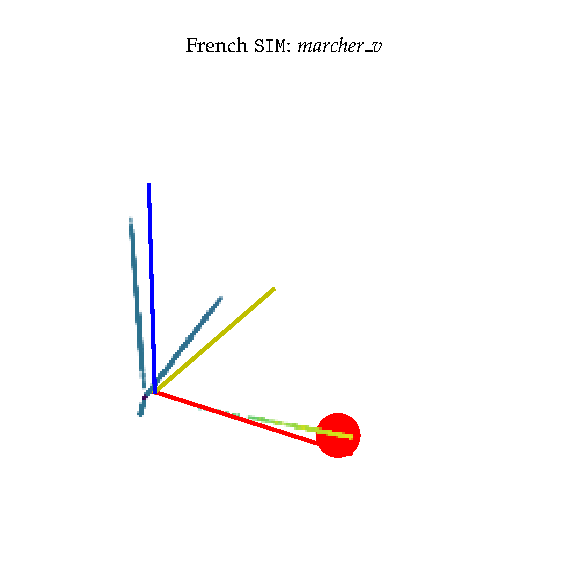
\includegraphics[scale=1]{Figures/FreSIMPCAformarcher_v.pdf}
        }
        \caption[French \code{SIM} Space Visualization]{Due to the nature of WOLF, 
        \code{SIM}'s first PCs denotes POS category. Light colors indicate the proximity of the represented words with \emph{marcher\_v}.}
        \label{fig:freSIMmarcher}
    \end{minipage}%
    \begin{minipage}[t]{.5\textwidth}
        \centering
        \makebox[.5\linewidth]{
        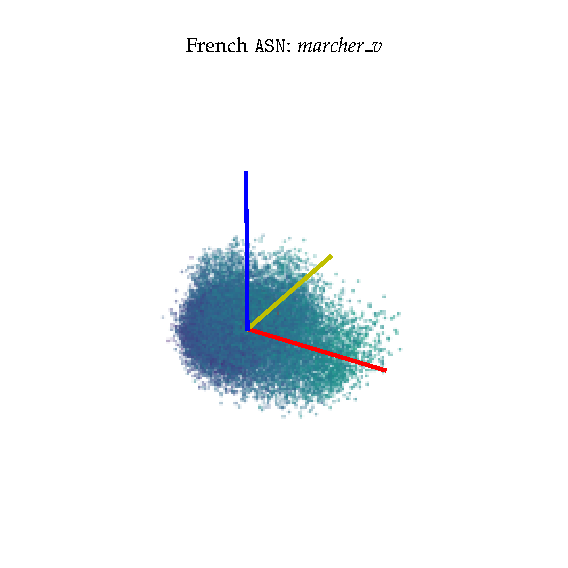
\includegraphics[scale=1]{Figures/FreASNPCAformarcher_v.pdf}
        }
        \caption[French \code{ASN} Space Visualization]{\code{ASN}'s variance are more homogeneously distributed over PCs.}
        \label{fig:freASNmarcher}
    \end{minipage}
\end{figure}


\begin{figure}
    \centering
    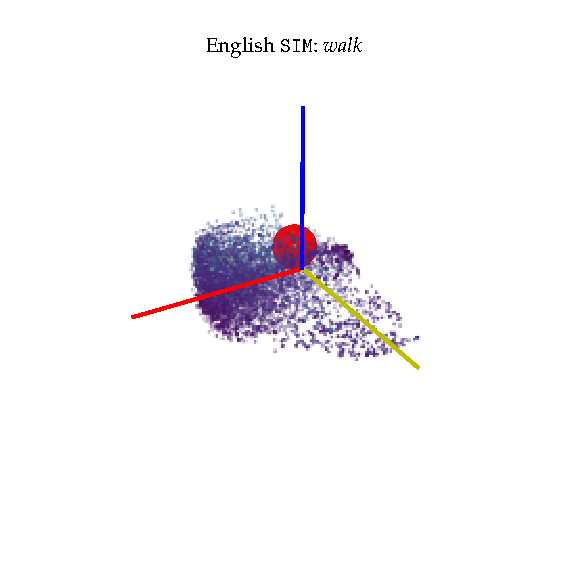
\includegraphics[scale=1]{Figures/EngSIMPCAforwalk.pdf}
    \caption[English \code{SIM} Space Visualization]{English's \code{SIM} however seems not to be macroscopically influenced by POS information.}
    \label{fig:engSIMwalk}
\end{figure}

\subsection{Semantic Ranking Task Results}
\label{appsubsec:wnembeddingtests}
\begin{table}
 \centering
 \begin{ThreePartTable} 
\begin{tabularx}{\textwidth}{p{3cm} *{2}{p{.5cm}} *{2}{p{1.7cm}} *{4}{L}} 
\multicolumn{8}{l}{\tabhead{English \code{WordNetEmbedding} Iterations}} \\
 \toprule
 \mr{2}{=}{\tabhead{Relations}} & \mr{2}{=}{\rotatebox[origin=c]{90}{\tabhead{Lexicon}}} & \mr{2}{=}{\rotatebox[origin=c]{90}{\tabhead{Dim.}}} & \mr{2}{=}{\tabhead{Metric}}  & \mc{3}{l}{\tabhead{\emph{Similarity}}} & \tabhead{\emph{Association}} \\
 \cmidrule{5-7}
 & & & & \small{\textbf{SIMLEX-999}} & \small{\textbf{WS353-SIM}} & \small{\textbf{RG1965}} & \small{\textbf{WS353-ASN}} \\
 \toprule
 \mr{4}{=}{\textbf{S}ynonymy} &\mr{2}{=}{15k}  & \mr{12}{=}{850} & Pearson & .2256 & .2679 & .3627 & .123 \\
 & & & Spearman & .2001 & .2003 & .3403 & .0971 \\
\cmidrule{2-2} \cmidrule{4-8}
  & \mr{2}{=}{60k} &  & Pearson & .234 & .2112 & .3394 & .1449 \\
 & & & Spearman & .1747 & .1895 & .2629 & .1129 \\
 \cmidrule{1-2} \cmidrule{4-8}
 \mr{2}{=}{S+Antonymy} & \mr{6}{=}{15k} &  & Pearson & .1534 & .2743 & .373 & .0969 \\
 & & & Spearman & .1255 & .1922 & .3302 & .0817 \\
 \cmidrule{1-1} \cmidrule{4-8}
 \mr{2}{=}{S+\textbf{H}yp\textbf{e}r/\textbf{H}yp\textbf{o}nymy} &  &  & Pearson & .3904 & .4825 & .6187 & .0373 \\
 & & & Spearman & .4018 & .3856 & .5145 & .0259 \\
 \cmidrule{1-1} \cmidrule{4-8}
 \mr{6}{=}{SHeHo+ adj.participle\_of\_verb+ adj.similar+ adv.derive\_from\_adj} &  &  & Pearson & .5079 & .5333 & .6784 & .0525 \\
 & & & Spearman & .4986 & .4214 & .576 & .0272 \\
 \cmidrule{2-2} \cmidrule{4-8}
  & \mr{2}{=}{60k} &  & Pearson & .5268 & .5483 & .6991 & .1092 \\
 & & & Spearman & .5152 & .4757 & .5501 & .0515 \\
 \cmidrule{2-8}
  & \mr{2}{=}{15k\tnote{0}}  & \mr{2}{=}{511} & Pearson & .506 & & & .0279 \\
 & & & Spearman & .4989 & & & .0193 \\
 \cmidrule{2-8} 

&  & \mc{2}{r}{Out Of Vocabulary} & .002 & .02 & 0 & .012 \\
\midrule
\mr{4}{=}{All\tnote{1}} & \mr{2}{=}{13k\tnote{2}} & \mr{8}{=}{850} & Pearson & .5 & .65 & .65 & .32 \\
 & & & Spearman & .52 & .67 & .75 & .33 \\
\cmidrule{2-2} \cmidrule{4-8}
 & \mr{2}{=}{60k\tnote{3}} & & Pearson & .5 & .51 & .56 & .31 \\
 & & & Spearman & .51 & .58 & .72 & .3 \\
\cmidrule{1-2} \cmidrule{4-8}
 \mr{3}{=}{Synonym Database\tnote{4}} & \mr{2}{=}{60k\tnote{5}} &  & Pearson & .6814 & .5819 & .8155 & .317 \\
 & & & Spearman & .6566 & .4677 & .7032 & .3153 \\
 \cmidrule{2-8}
 & & \mc{2}{r}{Out Of Vocabulary} & .066 & .227 & .077 & .19 \\
\bottomrule
\end{tabularx}
\begin{tablenotes}
    \footnotesize
    \item[0] Version reported in Table \ref{tab:engdecorrelationscores}.
    \item[1] Data reported by \textcite{saediWordNetEmbeddings2018}.
    \item[2] Cue words selected from psycholinguistic experiment datasets.
    \item[3] Words selected randomly. On the contrary, our implementation selects the top 60k most frequent words in \code{WordNet}. 
    \item[4] Synonym database is created by thesauri fusion and symmetrization. Data provided by \textcite{plouxModelMatchingSemantic2003}.
    \item[5] The synonym database contains multi-word phrases, whereas task benchmarks only test for single-word pairs. The actual lexicon size of the database is 36718.
\end{tablenotes}
\end{ThreePartTable}
\caption[English \code{WordNetEmbedding} Iterations]{Placeholder \label{apptab:engWordNetIteration}}
\end{table}

% \begin{table}
%     \centering
%     \begin{ThreePartTable} 
%    \begin{tabularx}{\textwidth}{p{3cm} *{3}{R} *{4}{L}} 
% \multicolumn{8}{l}{\tabhead{English Dissociation}} \\
%  \toprule
%  \mr{2}{=}{Common Crawl} & 2.2M, cased & 300 & Pearson & .3946 & .6573 & .6812 & .6091 \\
%  & & & Spearman & .3752 & .6298 & .6577 & .5709 \\
%  & & & OOV & .1 & 0 & 0 & 0 \\
%  \mr{2}{=}{CommonCraw - 01-23 Sim} & 8157 & 300 & Pearson & .1953 & .5854 & .5547 & .5633 \\
%  & & & Spearman & .2133 & .5719 & .5641 & .5918 \\
%  & & & OOV & & & & \\
%  \bottomrule
% \end{tabularx}
% \end{ThreePartTable}
% \caption[English Semantic Space Dissociation]{Placeholder \label{apptab:engDissociation}}
% \end{table}

\subsection{Vocabulary Coverage by POS}
\begin{table}
    \centering
    \begin{ThreePartTable}  
    \begin{tabularx}{\textwidth}{L *{10}{R}}
    \multicolumn{11}{l}{\tabhead{The Little Prince Vocabulary Coverage}} \\
    \toprule
    &  & \multicolumn{9}{l}{\tabhead{\# Instances in fMRI Recording Session}} \\
    \toprule
    &  & \tabhead{R1} & \tabhead{R2} & \tabhead{R3}& \tabhead{R4}& \tabhead{R5}& \tabhead{R6}& \tabhead{R7}& \tabhead{R8}& \tabhead{R9}\\
    \toprule
    \multicolumn{11}{l}{\tabhead{Nouns}} \\
    \toprule
    \mr{2}{*}{Story} & \textbf{T} &  269 & 286 & 306 & 242 & 284 & 355 & 281 & 265 & 246 \\
     & \textbf{V} & 142 & 140 & 152 & 107 & 108 & 147 & 109 & 135 & 121 \\
    \midrule
    \mr{4}{*}{\parbox{0.8cm}{\code{SIM} 56665}} & TM & 17 & 3 & 7 & 5 & 14 & 14 & 11 & 11 & 16 \\
     & \% & 6.32 & 1.05 & 2.29 & 2.07 & 4.93 & 3.94 & 3.91 & 4.15 & 6.50 \\
     & VM & 10 & 3 & 6 & 3 & 3 & 8 & 6 & 7 & 7 \\
     & \% & 7.04 & 2.14 & 3.95 & 2.80 & 2.78 & 5.44 & 5.50 & 5.19 & 5.79 \\
    \midrule
    \mr{4}{*}{\parbox{0.8cm}{\code{ASN} /\code{MIX} /\code{SIG} 24519}} & TM & 20 & 9 & 8 & 10 & 22 & 16 & 11 & 13 & 17 \\
     & \% & 7.43 & 3.15 & 2.61 & 4.13 & 7.75 & 4.51 & 3.91 & 4.91 & 6.91 \\
     & VM & 12 & 5 & 7 & 4 & 7 & 10 & 6 & 8 & 8 \\
     & \% & 8.45 & 3.57 & 4.61 & 3.74 & 6.48 & 6.80 & 5.50 & 5.93 & 6.61 \\
     \toprule
    \multicolumn{11}{l}{\tabhead{Verbs}} \\
    \toprule
    \mr{2}{*}{Story} & \textbf{T} & 227 & 274 & 313 & 306 & 258 & 296 & 331 & 278 & 335 \\
     & \textbf{V} & 104 & 109 & 142 & 119 & 84 & 113 & 99 & 110 & 118 \\
    \midrule
    \mr{4}{*}{\parbox{0.8cm}{\code{SIM} 56665}} & TM & 9 & 15 & 14 & 15 & 10 & 4 & 7 & 12 & 7 \\
     & \% & 3.96 & 5.47 & 4.47 & 4.90 & 3.88 & 1.35 & 2.11 & 4.32 & 2.09 \\
     & VM & 7 & 7 & 9 & 11 & 9 & 4 & 5 & 8 & 6 \\
     & \% & 6.73 & 6.42 & 6.34 & 9.24 & 10.71 & 3.54 & 5.05 & 7.27 & 5.08 \\
    \midrule
    \mr{4}{*}{\parbox{0.8cm}{\code{ASN} /\code{MIX} /\code{SIG} 24519}} & TM & 9 & 19 & 15 & 17 & 10 & 8 & 9 & 12 & 14 \\
     & \% & 3.96 & 6.93 & 4.79 & 5.56 & 3.88 & 2.70 & 2.72 & 4.32 & 4.18 \\
     & VM & 7 & 10 & 10 & 13 & 9 & 7 & 6 & 8 & 10 \\
     & \% & 6.73 & 9.17 & 7.04 & 10.92 & 10.71 & 6.19 & 6.06 & 7.27 & 8.47 \\
     \toprule
     \multicolumn{11}{l}{\tabhead{Adjectives \& Adverbs}} \\
     \toprule
     \mr{2}{*}{Story} & \textbf{T} & 229 & 252 & 241 & 214 & 190 & 251 & 207 & 169 & 221 \\
     & \textbf{V} & 102 & 111 & 117 & 103 & 100 & 107 & 94 & 83 & 104 \\
     \midrule
     \mr{4}{*}{\parbox{0.8cm}{\code{SIM} 56665}} & TM & 10 & 12 & 11 & 7 & 6 & 15 & 6 & 7 & 4 \\
      & \% & 4.37 & 4.76 & 4.56 & 3.27 & 3.16 & 5.98 & 2.90 & 4.14 & 1.81 \\
     & VM & 9 & 6 & 7 & 6 & 4 & 7 & 5 & 4 & 3 \\
     & \% & 8.82 & 5.41 & 5.98 & 5.83 & 4.00 & 6.54 & 5.32 & 4.82 & 2.88 \\
     \midrule
     \mr{4}{*}{\parbox{0.8cm}{\code{ASN} /\code{MIX} /\code{SIG} 24519}} & TM & 19 & 19 & 15 & 10 & 16 & 36 & 15 & 12 & 10 \\
      & \% & 8.30 & 7.54 & 6.22 & 4.67 & 8.42 & 14.34 & 7.25 & 7.10 & 4.52 \\
      & VM & 11 & 11 & 9 & 8 & 10 & 15 & 8 & 6 & 7 \\
      & \% & 10.78 & 9.91 & 7.69 & 7.77 & 10.00 & 14.02 & 8.51 & 7.23 & 6.73 \\
    \bottomrule
    \end{tabularx}
    \end{ThreePartTable}
    \caption[The Little Prince Vocabulary Coverage by POS]{\textbf{T}: Token, \textbf{V}: Lexicon Unit, M: Miss\label{apptab:lppcoverage}}
    \end{table}


\subsection{Corpus-Targeted Semantic Feature Selection}
[TODO still necessary?]


\section{Non-nested Model Comparison}
\label{appsubsec:nonnestedcompres}

\subsubsection{Use \code{SIM} to Predict \code{ASN}}
[TODO, insert heat-map of coefficients]
Each of the 203 columns in the \code{ASN} class design matrix (including non-semantic features) are predicted by 103 columns of the \code{SIM} class design matrix. We averaged the \code{r2} score of each column model across 9 cross-validation runs. The histogram of the scores are plotted in Figure \ref{fig:SIMASNDist}, informative model scores are presented in Table \ref{tab:SIMASNScores}. As our design-matrices are orthonormalized, columns sitting at larger indexes have a dependency on smaller-indexed columns. The first columns being bell predicted start at index 12 (to 14). Other columns are scattered up to index 47. We can therefore conclude that the predictability found are purely due to numerical coincidences.

\begin{figure}
    \centering
    \begin{minipage}[t]{.5\textwidth}
        \centering
        \makebox[.5\linewidth]{
            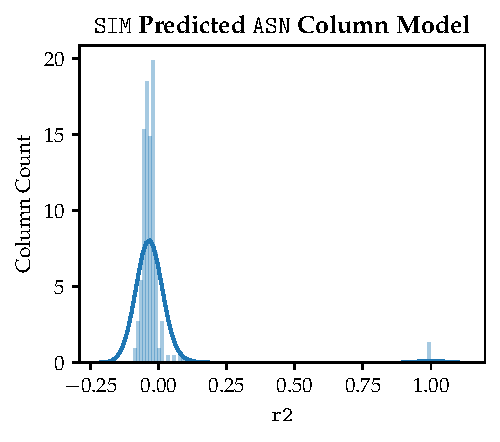
\includegraphics[scale=.8]{Figures/SIMASNDist.pdf}
            }
            \caption[\texttt{SIM} Predicted \texttt{ASN} Column Model]{3 columns are perfectly predicted as they are non-semantic features that are shared by the design matrices. For the rest most of the column-models are worse than arbitrary models.} 
            \label{fig:SIMASNDist}
    \end{minipage}%
    \begin{minipage}[t]{.5\textwidth}
        \centering
        \makebox[.5\linewidth]{
            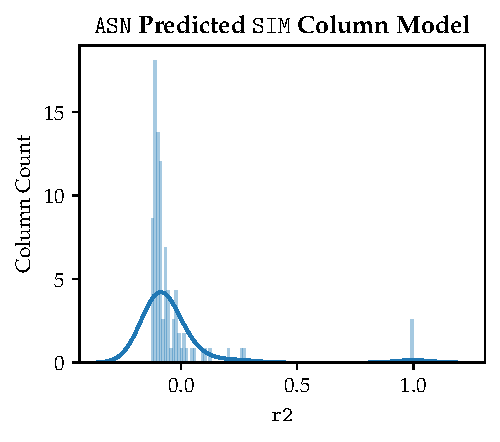
\includegraphics[scale=.8]{Figures/ASNSIMDist.pdf}
            }
            \caption[\texttt{ASN} Predicted \texttt{SIM} Column Model]{Most of the column-models are worse than arbitrary models. More columns in \code{SIM} are better predicted with \code{ASN} design matrices.} 
            \label{fig:ASNSIMDist}
    \end{minipage}
\end{figure}


\begin{table}
    \centering
    \begin{ThreePartTable}
    \begin{tabularx}{\textwidth}{p{1.7cm} *{11}{L}}
    \mc{12}{l}{\tabhead{\texttt{SIM} Predicted \texttt{ASN} Column Model Performances}} \\
    \toprule
    \tabhead{Col Index} & 22 & 20 & 14 & 37 & 47 & 18 & 27 & 26 & 13 & 12 & 30 \\  
    \tabhead{\code{r2}} & .0891 & .0834 & .0548 & .0346 & .0164 & .0152 & .0122 & .0113 & .0112 & .0075 & .0004 \\  
    \tabhead{\code{r}} & .2984 & .2887 & .2340 & .1861 & .1279 & .1233 & .1104 & .1064 & .1058 & .0867 & .0203 \\
    \bottomrule
    \end{tabularx}
    \end{ThreePartTable}
    \caption[\texttt{SIM} Predicted \texttt{ASN} Column Model Performances]{Index starts at 0, \code{ASN} group features starts from 3.  Among the 14 informative models (\code{r2} > 0), 3 are non-semantic features (not listed above). Pearson's \code{r} are converted from \code{r2}. \label{tab:SIMASNScores}}
\end{table}

\begin{table}
    \centering
    \begin{ThreePartTable}
    \begin{tabularx}{\textwidth}{p{1.7cm} *{11}{L}}
    \mc{12}{l}{\tabhead{\texttt{ASN} Predicted \texttt{SIM} Column Model Performances}} \\
    \toprule
    \tabhead{Col Index} & 6 & 3 & 5 & 11 & 4 & 7 & 75 & 18 & 42 & 25 & 47 \\  
    \tabhead{\code{r2}} & .2761 & .2646 & .2041 & .1256 & .1032 & .0971 & .0529 & .0485 & .0192 & .0158 & .0107 \\  
    \tabhead{\code{r}} & .5254 & .5144 & .4518 & .3544 & .3213 & .3116 & .2299 & .2202 & .1385 & .1256 & .1037 \\
    \bottomrule
    \end{tabularx}
    \end{ThreePartTable}
    \caption[\texttt{ASN} Predicted \texttt{SIM} Column Model Performances]{Index starts at 0, \code{SIM} group features starts from 3. \code{SIM} columns are much better predicted by \code{ASN}. \label{tab:ASNSIMScores}}
\end{table}

\subsubsection{Use \code{ASN} to Predict \code{SIM}}

The same procedure yields also 14 effective column models for \code{SIM}. The correlation coefficients are significantly higher than the models predicted with \code{SIM} matrices. Besides, the first 5 columns of \code{SIM} are all well predicted (\code{r} > 0.30) by \code{ASN}, indicating there's partial signal information overlap between the two models. Since Section \ref{appsubsec:projectorvisu} shows that the first 4 dimensions in \code{SIM} one-hot encode POS information, it is reasonable that POS information is also traceable in syntagmatic-information dominated semantic embedding.

To further investigate the column-wise correlation, we also plot the coefficients of each \code{ASN} column learned by GLM. [TODO heatmap average].

\section{Regression}
\subsection{More on \(\alpha\) and Dimension Selection}
\label{appsubsec:alphadim}

\subsubsection{Completeness of Research Space}

For illustrative purpose, we selected four typical voxels in post-hoc from the regression results of \code{MIX}, run 1 subject 1 (Figure \ref{fig:TypicalVoxelDistributionS1R1})\footnote{Interactive version of the plot available online \url{https://plot.ly/~neegola/11/}.}. \code{MIX} is used since it is the default semantic space used in other works and has not been modified. Each voxel is the best modeled voxel who maximizes \code{r2} among all \(\alpha\)s using only partial feature information of a certain regressor class. For example, a \code{CWRATE} class typical voxel is a voxel of which the best \code{r2} is achieved with \emph{all} first 3 features (\code{dim=3}). 

\begin{figure}
    \centering
    \makebox[\linewidth]{
    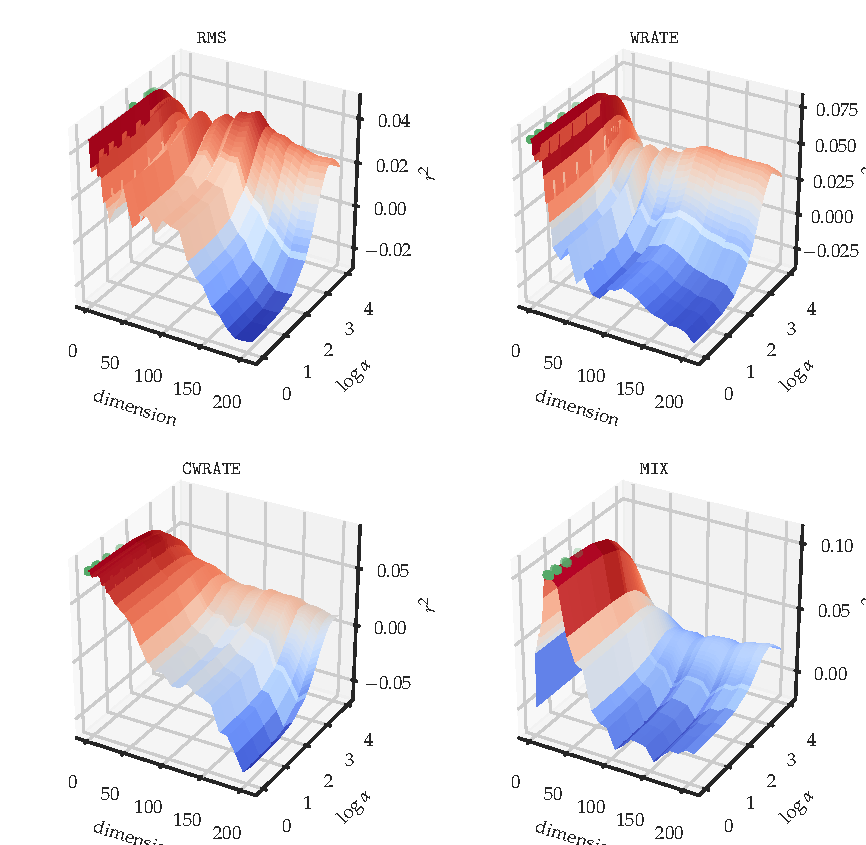
\includegraphics[scale=1]{Figures/TypicalVoxelDistributionS1R1.pdf}
    }
    \caption[Typical-Voxels' Response to \(\alpha\) and Dimension]{A selection of typical voxels found in \code{MIX} model regression results of subject 1 run 1. As shown by all four voxels, the regularization by large \(\alpha\) is beneficial only in higher feature dimensions. Our selection of \(\alpha\) contains a near-optimal value candidates for these voxels since the curve is all declining for the largest values. Green plots indicate the top 10 best configurations of the given voxel.} 
    \label{fig:TypicalVoxelDistributionS1R1}
\end{figure}

The optimal \code{r2}s of typical voxels are never attained at the upper bound of \(\alpha\) and dimension space. We plotted the heat-map for all voxels from the same run to verify if it is also the case at the whole-brain level (e.g. Figure \ref{fig:MIX_HeatmapAlphaDimS1R1}). We averaged 9 cross-validation run results to visualize subject-level best configuration distribution (Figure \ref{fig:MIX_HeatmapAlphaDimS1R0}). Histograms of best dimension and \(\alpha\) voxel-configuration of the averaged results are also plotted in Figure \ref{fig:MIX_CountPlotAlphaDimS1R0}. Plots for all runs and all subjects are available online\footnote{[TODO] add public url}. The analysis confirms that our parameter combination test range contains the near-optimal configuration for each voxel.

\begin{figure}
    \centering
    
    \makebox[.5\linewidth]{
            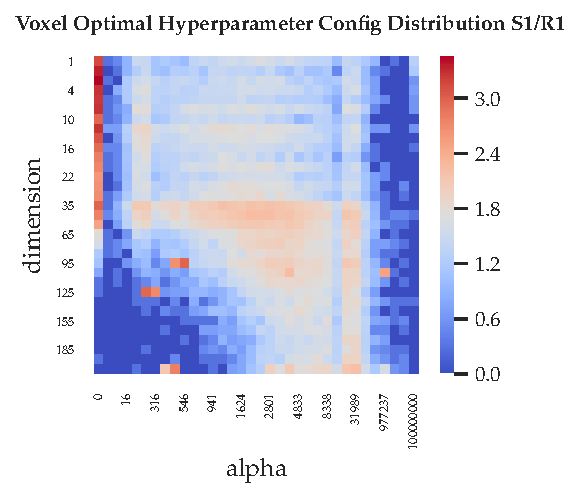
\includegraphics[scale=.8]{Figures/MIX_HeatmapAlphaDimS1R1.pdf}
            }
            \caption[Session Best Hyper-parameter Configuration Voxel-Count Heat-map]{[TODO fix title display] The scores are retrieved from \code{MIX} model regression for subject 1, fMRI run 1. Each cell represents an \(\alpha\) and dimension combination. The color indicates the logarithm of number of voxels having its global optimality with a given parameter set after having filtered out non-informative voxels (\code{r2} < 0). For small dimensions (< 35), small \(\alpha\)s (including 0) achieve the best performance. Starting from dimension 35, Ridge regularization with larger \(\alpha\)s is necessary.} 
            \label{fig:MIX_HeatmapAlphaDimS1R1}
   
\end{figure}

\begin{figure}
    \centering
    \makebox[\linewidth]{
    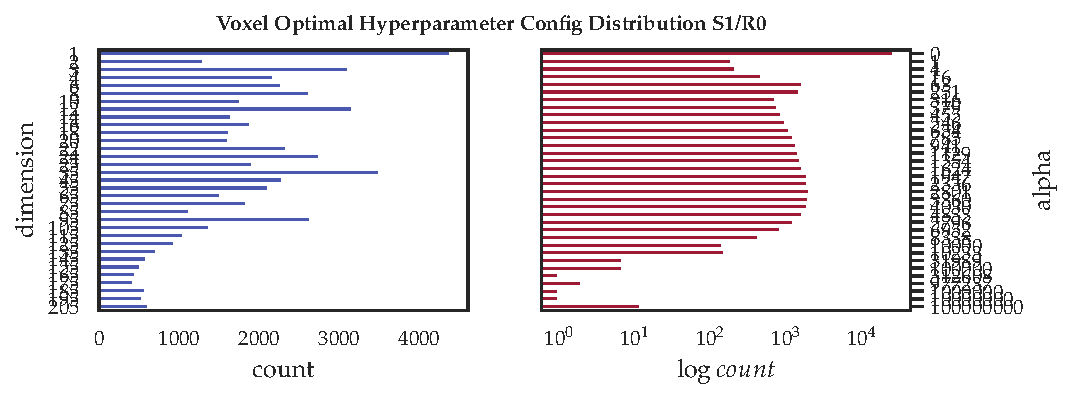
\includegraphics[scale=1]{Figures/MIX_CountPlotAlphaDimS1R0.pdf}
    }
    \caption[Best Hyper-parameter Configuration Voxel-Count Histograms]{[TODO, fix axis display] \textbf{Left panel}: Among informative voxels, a large portion of voxels are best modeled by \code{RMS} and \code{CWRATE} regressor classes. The addition of each semantic dimension from \code{MIX} improved a small proportion of voxel-models, marginal might be the contribution. \textbf{Right panel}: Most of the voxels are best modeled without Ridge regularization. The larger number obtained at \(\alpha=10000\) might indicate that larger alpha values might help better model a thousand voxels. A cumulation of voxel-count at the upper bound of the \(\alpha\) axis is noted: we performed post-hoc test for larger \(\alpha\) values than in the initial configuration, but the improvement of \code{r2} over the original score is marginal (\(<10^{-4}\)) for a sample of these voxels. A post-hoc analysis of larger \(\alpha\)s indicates a limited improvement of \code{r2}, thus for computational simplicity we kept the original Grid Search space of \(\alpha\).\label{fig:MIX_CountPlotAlphaDimS1R0}} 
    
\end{figure}

\subsubsection{\(\alpha\) Variability across Voxels}
[TODO: histogram animation with alpha evolution, ]

[TODO: discussion on overfit by dimension, despite regularization]




\subsection{Impact of \code{CWRATE}}
[TODO: Taking over SIM/ASN ? Visualize regression results without CWRATE]

\section{Embedding Model Brain Maps}
\subsection{\code{SIM} and \code{ASN} F-test}
\begin{table}
    \small
    \centering
    \begin{ThreePartTable}
        \begin{tabularx}{\textwidth}{l l p{1.5cm} *{3}{r} *{2}{P{1.2cm}}P{1.4cm}}
            \mc{6}{l}{\tabhead{\code{ASN} Best Improved Voxel Clusters}} \\
    \toprule
    \tabhead{Position} & \tabhead{BA} & \tabhead{Functional Label} & \tabhead{x} & \tabhead{y} & \tabhead{z} & \tabhead{\# Voxel} & \(\Delta\)\code{r2} \tabhead{Peak} & \(-\log_{10}\)\tabhead{ p-value} \\
    
    \toprule
    \mc{7}{l}{\tabhead{Top 4.7\%}}  &  > .0065 & >4.18   \\
    \midrule
    Temporal Mid L & 37 & Fusiform & -53 & -58 & -3 & 131 & .0121 & 4.35\\
    Frontal Inf Tri L & 46 & - & -46 & 37 & 11 & 68 & .0124 & 4.35 \\
    Occipital Mid L & 39 & - & -32 & -78 & 41 & 242 & .0125 & 4.35 \\
    Frontal Sup Medial L & 9 & - & -5 & 58 & 32 & 32 & .0092 & 4.35 \\
    Cingulum Mid L & 31 & - & -1 & -36 & 43 & 34 & .0105 & 4.35  \\
    Frontal Mid R & 8 & - & 28 & 15 & 46 & 63 & .0093 & 4.35  \\
    Angular R & 39 & - & 43 & -75 & 39 & 191 & .0114 & 4.35  \\
    Temporal Mid R & 21 & - & 46 & -32 & 0 & 182 & .0106 & 4.35 \\
    Frontal Inf Tri R & 46 & - & 50 & 35 & 8 & 56 & .0107  & 4.35\\
\bottomrule
    \end{tabularx}
    % \begin{tablenotes}
    % \footnotesize
    % \item[1] A cosine distance near 0 indicates a greater similarity.
% \end{tablenotes}  
\end{ThreePartTable}
\caption[\code{ASN} Voxel Improvement Clusters]{The Wilcoxon signed-rank test's p-value is thresholded at \(10^{-4.18}\) to make a clean cut is found in p-value histogram. Only 13 voxels reach a significance level of \(10^{-4.35}\) as is done with \code{ASN}. The voxel selection leads to top 4.7\% important voxel-model improvements. The largest \code{r2} boost is found in left MOccipital, followed by right mSTS, right Angular, left pFusiform bilateral iTriFrontal. Relatively smaller clusters are found in MCingulum L, L S Frontal BA9, R M Frontal BA8.  \label{tab:asnImprovementClusters}}
\end{table}
\begin{table}
    \small
    \centering
    \begin{ThreePartTable}
    \begin{tabularx}{\textwidth}{L l L *{3}{r} *{1}{R}}
    \mc{6}{l}{\tabhead{\code{CWRATE/SIM/SIG/ASN} F-test Significant Voxels}} \\
    \toprule
    \tabhead{Position} & \tabhead{BA} & \tabhead{Functional Label} & \tabhead{x} & \tabhead{y} & \tabhead{z} & \tabhead{\# Voxel in Region}\\
    \toprule
\code{CWRATE} \\
\midrule
    Fusiform L & 19 & - & -30.0 & -71.0 & -13.0 & 1 \\
Occipital Mid R & 19 & - & 46.0 & -77.0 & 3.0 & 1 \\
Cerebelum 8 R & 37 & Fusiform & 24.0 & -42.0 & -45.0 & 1 \\
Cerebelum 9 R & 37 & Fusiform & 8.0 & -52.0 & -35.0 & 1 \\
Lingual R & 18 & VisualAssoc & 8.0 & -90.0 & -7.0 & 1 \\
Precuneus R & 7 & - & 5.0 & -55.0 & 75.0 & 1 \\
Cingulum Post R & 30 & - & 2.0 & -33.0 & 12.0 & 1 \\
Occipital Sup L & 7 & - & -24.0 & -83.0 & 44.0 & 1 \\
Fusiform L & 18 & VisualAssoc & -24.0 & -83.0 & -16.0 & 1 \\
Lingual L & 18 & VisualAssoc & -24.0 & -90.0 & -16.0 & 1 \\
Cerebelum Crus2 R & 37 & Fusiform & 46.0 & -74.0 & -42.0 & 1 \\
Occipital Inf R & 37 & Fusiform & 52.0 & -68.0 & -13.0 & 1 \\
Occipital Inf L & 18 & VisualAssoc & -30.0 & -87.0 & -4.0 & 1 \\
Cerebelum Crus1 L & 18 & VisualAssoc & -33.0 & -87.0 & -26.0 & 1 \\
Cerebelum 8 L & 20 & - & -43.0 & -52.0 & -51.0 & 1 \\
Cerebelum Crus2 L & 37 & Fusiform & -43.0 & -64.0 & -38.0 & 1 \\
Cerebelum Crus2 L & 37 & Fusiform & -46.0 & -61.0 & -45.0 & 2.0 \\
Occipital Mid L & 19 & - & -49.0 & -74.0 & -0.0 & 1 \\
Temporal Pole Mid L & 38 & - & -52.0 & 11.0 & -35.0 & 1 \\
Cerebelum Crus2 L & 37 & Fusiform & -52.0 & -52.0 & -42.0 & 1 \\
Temporal Inf L & 37 & Fusiform & -55.0 & -45.0 & -23.0 & 1 \\
Cerebelum Crus1 L & 19 & - & -30.0 & -71.0 & -26.0 & 1 \\
Cerebelum 8 R & 37 & Fusiform & 36.0 & -55.0 & -51.0 & 1 \\
Temporal Pole Mid L & 38 & - & -55.0 & 11.0 & -32.0 & 1 \\
Rolandic Oper L & 6 & - & -62.0 & 2.0 & 9.0 & 1 \\

\toprule
\code{SIM} \\
\midrule
Temporal Mid L & 39 & - & -65.0 & -52.0 & 3.0 & 1 \\
Heschl L & 4 & PrimMotor & -65.0 & -11.0 & 9.0 & 1 \\
Temporal Mid L & 21 & - & -58.0 & -49.0 & 9.0 & 1 \\
Temporal Mid L & 39 & - & -55.0 & -55.0 & 3.0 &  1 \\
Temporal Sup R & 22 & - & 43.0 & -39.0 & 12.0 &  1 \\
\toprule
\code{SIG}\\
\midrule
Rolandic Oper R & 40 & - & 55.0 & -14.0 & 12.0 &  1 \\
Temporal Sup R & 22 & - & 58.0 & -30.0 & 3.0 &  1 \\
Temporal Sup R & 40 & - & 62.0 & -20.0 & 12.0 &  1 \\

\toprule
\code{ASN} \\
\midrule
Lingual R & 19 & - & 21.0 & -64.0 & -0.0 &  1 \\
Occipital Mid R & 18 & VisualAssoc & 33.0 & -80.0 & -0.0 &  1 \\

\bottomrule
    \end{tabularx}
    % \begin{tablenotes}
    % \footnotesize
    % \item[1] A cosine distance near 0 indicates a greater similarity.
% \end{tablenotes}  
\end{ThreePartTable}
\caption[\code{CWRATE/SIM/SIG/ASN} F-test Significant Voxels]{The most severe voxel score selection of \code{RMS} leads to left primary cortex (BA41) activation. Also well modeled voxels are distributed in more extensive areas of bilateral BA41 and right BA23 and BA10. With the addition of \code{CWRATE} features, voxel performances are systematically improved. With \code{CWRATE}, no other clusters appear in the thresholded voxel set. Left BA41 has a higher concentration of best modeled voxels, while right BA41 and cingulum mid R [TODO labels] degrade in voxel score ranking. Right BA10 also improves in ranking. \label{tab:Ftest}}
\end{table}

\subsection{\code{SIG} Nested Model and Contrast} 
\label{subsec:sig}
[TODO: replace SIM by SIG]

\begin{figure}
    \centering
    \makebox[\linewidth]{
    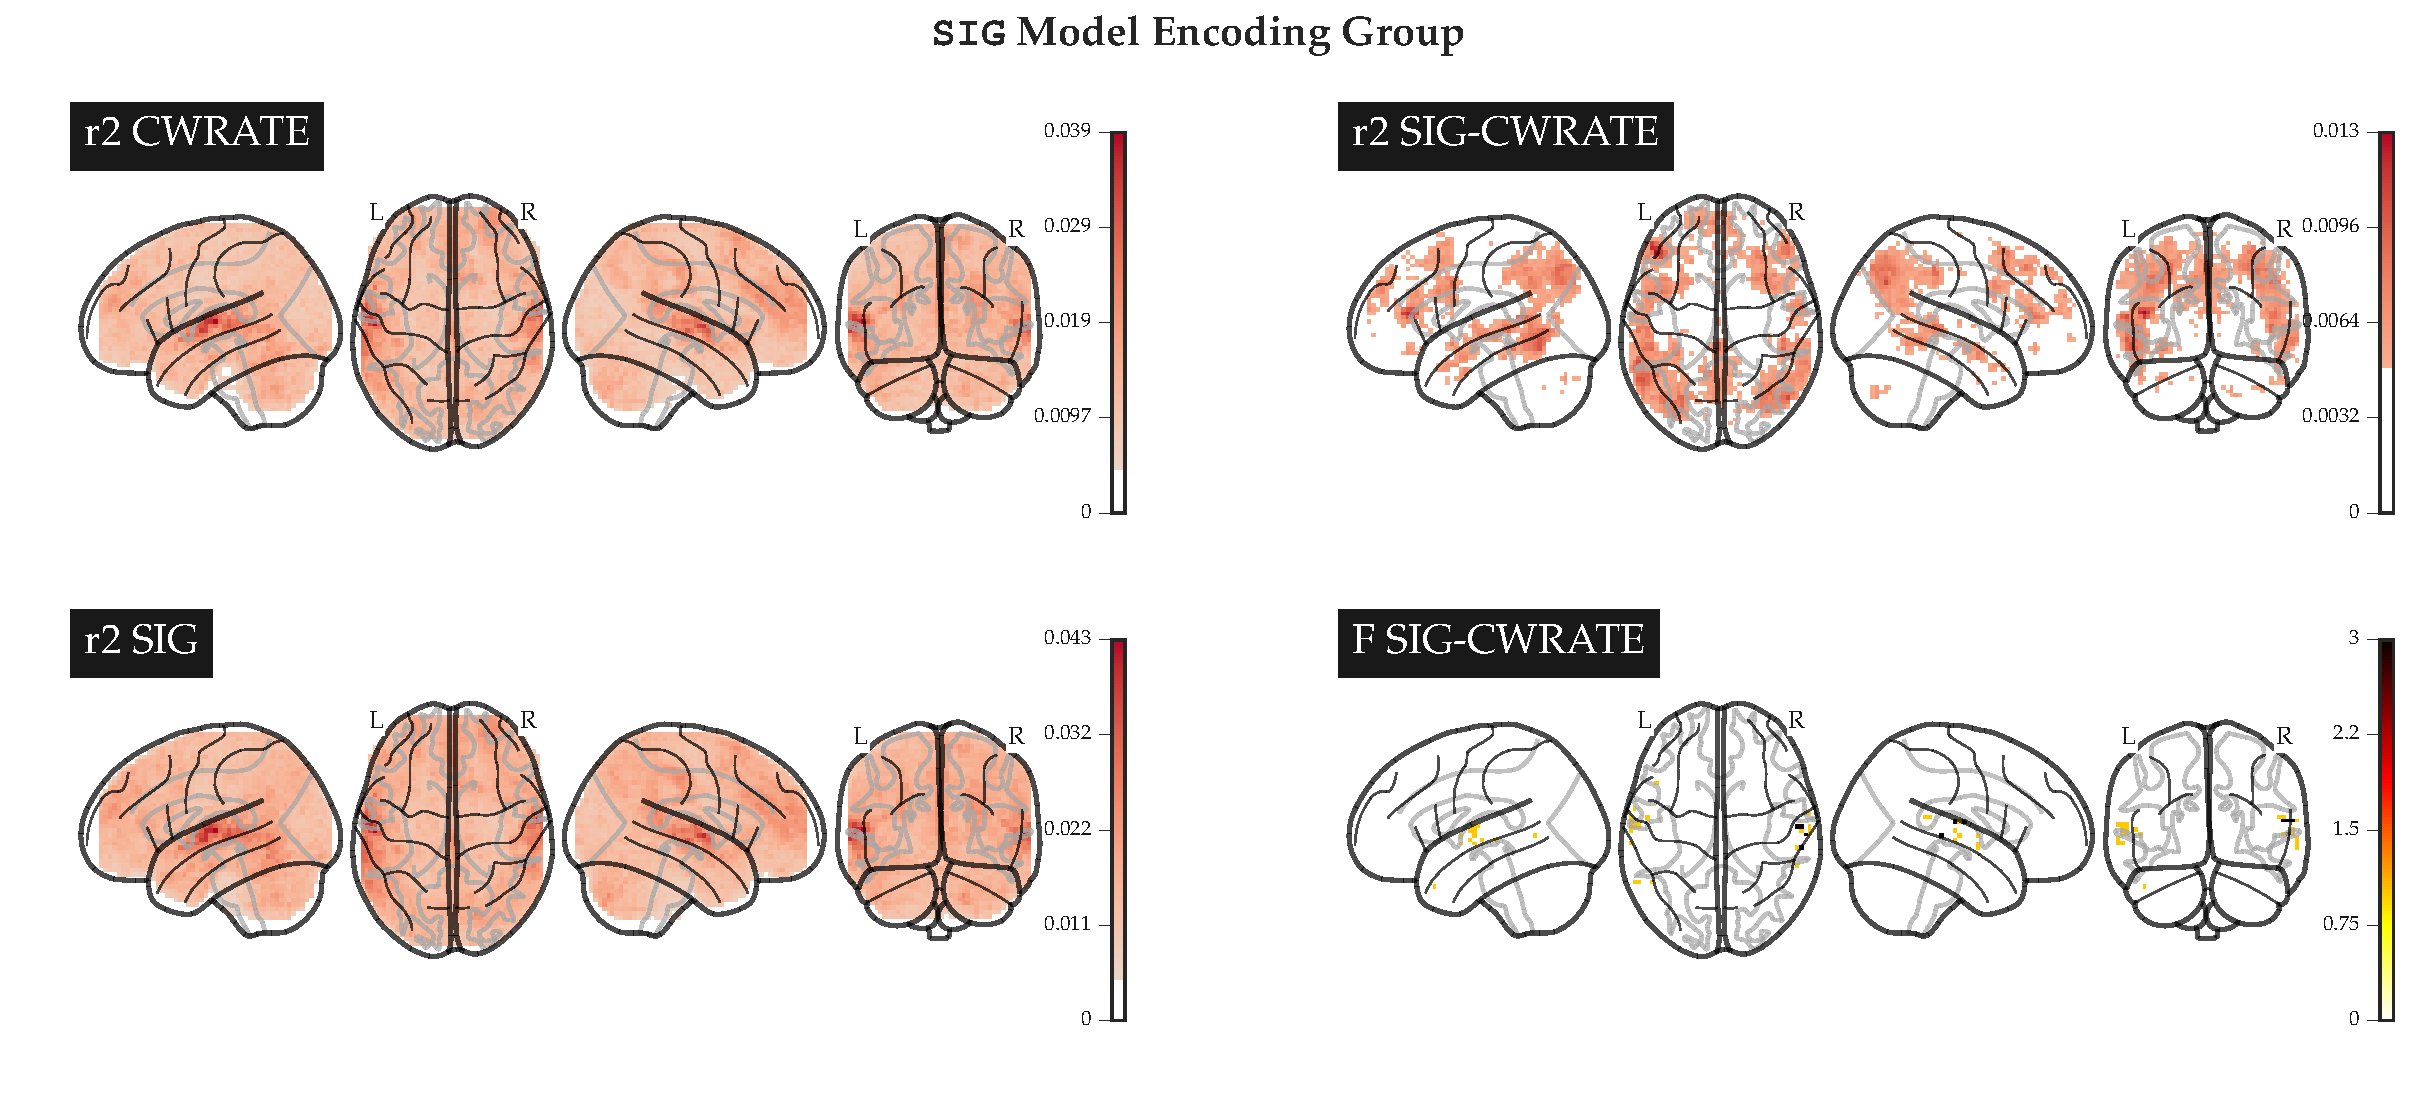
\includegraphics[width=.8\paperwidth]{Figures/SIG_ContrastMapG.pdf}
    }
    \caption[Encoding with \code{SIG} Features, Group]{[TODO]\textbf{Left panels}: The global activation pattern is unchanged with the feature addition. Best modeled zones are bilateral primary auditory cortices. \textbf{Right upper panel}  shows that \code{SIM} better models bilateral MTG, sup Parietal, Angular Gyrus (part of Wernicke's area), supramarginal gyrus and prefrontal areas (Table \ref{tab:simImprovementClusters}). F-test in \textbf{right lower panel} reports significant voxels in left pMTG BA21, 39, right pSTG BA22 and left Heschl BA4 (Table \ref{tab:Ftest}). Subject-wise results are available online at \url{http://bit.ly/micipsa_sim_wholebrain}.} 
    \label{fig:SIG_ContrastMapG}
\end{figure}


\begin{table}
    \small
    \centering
    \begin{ThreePartTable}
        \begin{tabularx}{\textwidth}{l l p{1.5cm} *{3}{r} *{2}{P{1.2cm}}P{1.4cm}}
            \mc{6}{l}{\tabhead{\code{SIG} Best Improved Voxel Clusters}} \\
    \toprule
    \tabhead{Position} & \tabhead{BA} & \tabhead{Functional Label} & \tabhead{x} & \tabhead{y} & \tabhead{z} & \tabhead{\# Voxel} & \(\Delta\)\code{r2} \tabhead{Peak} & \(-\log_{10}\)\tabhead{ p-value} \\
    \toprule
    \mc{7}{l}{\tabhead{Top .5\%}}  &  >.0079 & >4.35   \\
    \midrule
    Temporal Inf L & 37 & Fusiform & -56 & -56 & -12 & 85 & .0104 &4.35 \\
Frontal Inf Tri L & 46 & - & -46 & 35 & 12 & 35 & .0128 &4.35 \\
Parietal Sup L & 7 & - & -27 & -73 & 44 & 27 & .0093&4.35  \\
Angular R & 39 & - & 49 & -70 & 35 & 89 & .0105 &4.35 \\
Frontal Inf Tri R & 46 & - & 48 & 38 & 9 & 17 & .0088&4.35  \\
\bottomrule
    \end{tabularx}
    % \begin{tablenotes}
    % \footnotesize
    % \item[1] A cosine distance near 0 indicates a greater similarity.
% \end{tablenotes}  
\end{ThreePartTable}
\caption[\code{SIG} Voxel Improvement Clusters]{We thresholded Wilcoxon signed-rank test's significance at \(10^{-4.35}\) as a clean cut is found in p-value histogram, which leads to a selection of top .5\% important voxel-model improvements. The most significant and extensive cluster is found in left ITG, lateral Fusiform Gyrus, bilateral IFGtri (Broca's area), right angular gyrus (Wernicke's) and superior parietal gyrus. \label{tab:sigImprovementClusters}}
\end{table}
[SIG 209, No particularly different results are found. in PeaksSIG.ipynb]

[TODO, SIM->SIG]
We added with upon non semantic-embedding models \code{SIM} freatures to construct \similarity semantic models. While the whole-brain activation pattern stays globally unchanged (Figure \ref{fig:SIM_ContrastMapG} for group-wise average), in \code{SIM} voxel-models, left primary cortex are better ranked than in \code{BASE} model, while right mid cingulum models degrade (Table \ref{tab:rmsCluters}). \code{SIM} enlarges the performance superiority of left STG over right STG, indicating a left preference for textual semantic \similarity processing. The shrinkage of Mid Cingulum's proportion in top 1\% voxel models might imply that it has a limited participating in \similarity processing. The \code{r2} distribution analysis (Figure \ref{fig:SIM_ASN_Distribution} left) shows that in group-average \code{SIM} is informative for most of the voxel-models and none of voxels is overfitted by this addition. Table \ref{tab:simImprovementClusters} reports the most improved voxel clusters by \code{SIM} to be located in bilateral MTG, left Sup Parietal and right Angular Cortex (W=210, \(\Delta\)\code{r2}>0.0079, p-value<\(10^{-4.35}\) uncorrected). Left MTG improvements are more extensive and more important than right MTG. F-test results shows that \code{SIM} significantly improves isolated voxels (Table \ref{tab:Ftest}, p-value<0.05 voxel-wise multi-comparison corrected) in left pMTG BA21, 39, right pSTG BA22.


\subsubsection{With \code{SIG}}
\begin{figure}
    \centering
    \makebox[\linewidth]{
    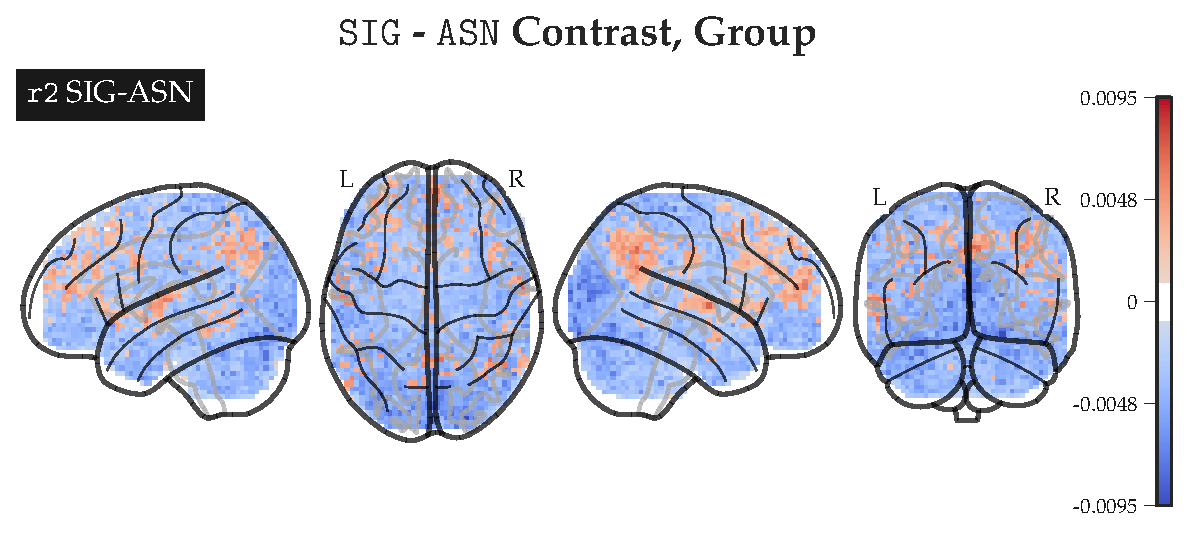
\includegraphics[width=.4\paperwidth]{Figures/EMB_SIG_ASN_r2_ContrastMapG.pdf}
    }
    \caption[\code{SIG}-\code{ASN} Contrast, Group]{[TODO]The differences of best voxel-model \code{r2}s are plotted. \code{SIM} preference is found in left BA10 SPFC, l aCC, l STS, l MPFC, r IParietal, r STG, MTG (Table \ref{tab:simasnContrastClusters_sim}) ... \code{ASN} preferences are found in bilateral BA18, RBA2-, l BA7 SParietal, R bA18, l BA37, l BA19, (visual association, fusimorm, primary visual, Parahip, and Thalamus). Subject-wise results are available online at \url{http://bit.ly/micipsa_sig_asn_contrast}} 
    \label{fig:EMB_SIG_ASN_ContrastMapG}
\end{figure}

\begin{table}
    \small
    \centering
    \begin{ThreePartTable}
        \begin{tabularx}{\textwidth}{l l p{1.6cm} *{3}{r} *{2}{P{.8cm}} P{1.3cm} P{.5cm}}


    \mc{6}{l}{\tabhead{\code{SIG-ASN} Voxel Contrast, Preference for \code{SIG}}} \\
    \toprule
    \tabhead{Position} & \tabhead{BA} & \tabhead{Functional Label} & \tabhead{x} & \tabhead{y} & \tabhead{z} & \tabhead{\# Voxel} & \(\Delta\)\code{r2} \tabhead{Peak} & \(-\log_{10}\)\tabhead{ p-value} & \tabhead{Cluster ID} \\
    \toprule

    Angular R & 39 & - & 39 & -55 & 28 & 8 &6.74&.0078& 1 \\
    Precuneus R & 31 & - & 8 & -55 & 41 & 13 &6.41&.0075& 2 \\
    Precuneus R & 23 & - & 8 & -55 & 25 & 4 &6.15&.0073& 3 \\
    \midrule
    Cingulum Ant L & 32 & - & -2 & 30 & 31 & 14 &5.94&.0072& 4 \\
    Cingulum Ant L & 32 & - & -11 & 34 & 22 &   &4.06&.0054& 4a \\
    Frontal Mid L & 10 & - & -36 & 49 & 15 & 3 &5.69&.0070& 5 \\
    Temporal Sup R & 41 & PrimAudi & 49 & -23 & 6 & 5 &5.45&.0068& 6 \\
    Precuneus L & 23 & - & -2 & -49 & 37 & 14 &5.38&.0067& 7 \\
    Cingulum Post L & 23 & - & -8 & -49 & 31 &   &3.81&.0052& 7a \\
    Caudate R & 48 & Caudate & 17 & 21 & 3 & 4 &5.38&.0067& 8 \\
    Frontal Sup Medial R & 10 & - & 5 & 56 & 15 & 4 &5.38&.0067& 9 \\
    Temporal Sup L & 41 & PrimAudi & -58 & -14 & 6 & 8 &5.30&.0066& 10 \\
    Precentral R & 8 & - & 39 & 8 & 44 & 2 &5.28&.0065& 11 \\
    Frontal Sup L & 10 & - & -27 & 59 & 25 & 2 &5.22&.0065& 12 \\
    Precentral L & 6 & - & -49 & 2 & 28 & 2 &5.03&.0063& 13 \\
    Temporal Sup L & 22 & - & -55 & -1 & -7 & 2 &4.98&.0062& 14 \\
    Temporal Inf L & 37 & Fusiform & -49 & -42 & -13 & 2 &4.77&.0060& 15 \\
    Temporal Sup R & 41 & PrimAuditory & 62 & -8 & 3 & 4 &4.70&.0060& 16 \\
    Cingulum Mid R & 23 & - & 5 & -20 & 34 & 6 &4.62&.0059& 17 \\
    Insula L & 47 & - & -36 & 18 & -13 & 2 &4.61&.0059& 18 \\
    Frontal Sup Medial R & 8 & - & 11 & 34 & 53 & 2 &4.57&.0059& 19 \\
    Angular R & 39 & - & 36 & -64 & 41 & 3 &4.57&.0059& 20 \\
    Caudate R & 48 & Caudate & 14 & 5 & 18 & 2 &4.46&.0058& 21 \\
    Parietal Sup L & 7 & - & -14 & -71 & 50 & 4 &4.46&.0058& 22 \\
    Temporal Mid L & 19 & - & -52 & -68 & 6 & 3 &4.29&.0056& 23 \\
    Frontal Inf Orb L & 47 & - & -46 & 21 & -7 & 2 &4.26&.0056& 24 \\
    Parietal Inf R & 40 & - & 46 & -42 & 41 & 2 &4.26&.0056& 25 \\
    Precentral R & 8 & - & 39 & 5 & 50 & 3 &4.24&.0056& 26 \\
    Cuneus L & 19 & - & -14 & -74 & 34 & 5 &4.05&.0054& 27 \\
    Frontal Sup Medial R & 10 & - & 5 & 62 & 12 & 3 &4.01&.0054& 28 \\
    Cingulum Mid L & 23 & - & -5 & -14 & 28 & 3 &4.00&.0054& 29 \\
    Cingulum Ant R & 32 & - & 5 & 43 & 3 & 3 &3.94&.0053& 30 \\
    Precuneus L & 7 & - & -14 & -68 & 31 & 2 &3.83&.0052& 31 \\
    Angular L & 39 & - & -46 & -64 & 47 & 2 &3.81&.0052& 32 \\
    Frontal Sup Medial R & 10 & - & 2 & 53 & 6 & 3 &3.79&.0052& 33 \\
    Frontal Sup Medial R & 10 & - & 8 & 59 & 22 & 5 &3.75&.0051& 34 \\
    Cingulum Mid L & 23 & - & -5 & -23 & 34 & 3 &3.74&.0051& 35 \\
    Precuneus L & 7 & - & -17 & -61 & 66 & 2 &3.73&.0051& 36 \\
    Frontal Sup Medial L & 9 & - & 2 & 56 & 34 & 2 &3.65&.0050& 37 \\
    Frontal Sup R & 8 & - & 21 & 37 & 53 & 2 &3.40&.0047& 38 \\
    Parietal Inf R & 40 & - & 43 & -45 & 44 & 2 &3.27&.0046& 39 \\
\bottomrule
    \end{tabularx}
    \begin{tablenotes}
            \footnotesize
            \item Voxel-wise Bonferroni corrected p=0.05 corresponds to uncorrected \(-\log_{10}\) p=6.04.
            % \item[*] Sub-peaks in one same cluster. 
        \end{tablenotes}  
    % \footnotesize
    % \item[] A cosine distance near 0 indicates a greater similarity.
% \end{tablenotes}  
\end{ThreePartTable}
\caption[\code{SIG-ASN} Voxel Contrast, \code{SIG}, Group]{The \code{SIG}-\code{ASN} contrast is computed by subtracting group-average voxel-wise \code{r2}. The significance is reported by two-tailed Wilcoxon signed-rank test before multi-comparison correction. The cluster is reported only if the average \code{r2} of \code{SIG} is higher than \code{ASN}. No cluster-size limit was applied when computing connected clusters. \code{SIG}'s model advantage over \code{ASN} is found in right angular gyrus and right medial parietal cortex. Left aSTG, right pSTG, left pITG, Frontal, limbic, parietal clusters are found significant before correction. \label{tab:sigasnContrastClusters_sig}}
\end{table}

\begin{table}
    \small
    \centering
    \begin{ThreePartTable}
    \begin{tabularx}{\textwidth}{l l p{1.6cm} *{3}{r} *{2}{P{1cm}} P{1.4cm} P{.5cm}}
        
    \mc{6}{l}{\tabhead{\code{SIG-ASN} Voxel Contrast, Preference for \code{ASN}}} \\
    \toprule
    \tabhead{Position} & \tabhead{BA} & \tabhead{Functional Label} & \tabhead{x} & \tabhead{y} & \tabhead{z} & \tabhead{\# Voxel} & \(\Delta\)\code{r2} \tabhead{Peak} & \(-\log_{10}\)\tabhead{ p-value} & \tabhead{Cluster ID} \\
    \toprule
Calcarine L & 17 & PrimVisual & 2 & -87 & 6 & 26 & - & 10.26 & 1 \\
Calcarine R & 17 & PrimVisual & 5 & -80 & 12 &   & .0095  & 8.30 & 1a \\
Cingulum Mid R & 32 & - & 17 & 5 & 37 & 2 & .0078 & 6.81  & 2 \\
Calcarine L & 18 & VisualAssoc & -2 & -99 & 12 & 2 & .0075& 6.27  & 3 \\
\midrule
Frontal Inf Orb R & 47 & - & 30 & 27 & -23 & 2 & .0065  & 5.25  & 4 \\
\bottomrule
    \end{tabularx}
    \begin{tablenotes}
        \footnotesize
        \item Voxel-wise Bonferroni corrected p=0.05 corresponds to uncorrected \(-\log_{10}\) p=6.04.
        % \item[*] Sub-peaks in one same cluster. 
    \end{tablenotes}  
    % \begin{tablenotes}
    % \footnotesize
    % \item[1] A cosine distance near 0 indicates a greater similarity.
% \end{tablenotes}  
\end{ThreePartTable}
\caption[\code{SIG-ASN} Voxel Contrast, \code{ASN}, Group]{The \code{SIG}-\code{ASN} contrast is computed by subtracting group-average voxel-wise \code{r2}. The significance is reported by two-tailed Wilcoxon signed-rank test before multi-comparison correction. The cluster is reported only if the average \code{r2} of \code{ASN} is higher than \code{SIG}. No cluster-size limit was applied when computing connected clusters. \label{tab:sigasnContrastClusters_asn}}
\end{table}



Section \ref{appsubsec:nonnestedcompres} suggests that first feature dimensions of \code{SIM} can be partially recovered by \code{ASN} model. Therefore, \code{ASN} might also be able to model voxels using less than 5 features from \code{SIM}, the result might thus lack low-level \code{SIM}/\code{ASN} contrast. As the first 4 dimensions of \code{SIM} encodes primarily POS information (Section \ref{appsubsec:projectorvisu}), we performed ad-hoc regressions on \code{SIM} space but uses only lemmas from a certain grammatical category to identify possible impacted regions. [TODO, supplementary]

The results found are consistent with the conjectures above: \code{ASN} scores are higher than \code{SIM} in average (Figure \ref{fig:SIM_ASN_Distribution} right), most of voxels respond better to \code{ASN} models (Figure \ref{fig:EMB_SIM_ASN_ContrastMapG}). As the Wilcoxon test shows (W=, \(\Delta\)\code{r2}>0.0068, p-value<0.05 voxel-wise multi-comparison corrected), only two significant clusters are found for \code{SIM} in ... (Table \ref{tab:simasnContrastClusters_sim}) and 17 are found for \code{ASN} (Table \ref{tab:simasnContrastClusters_asn}) in \dots.

The reported clusters for \code{SIM} are composed of 4 to 5 voxels. In our ROI analysis, ROIs larger than 26 voxels are used, thus none of the ROI revealed significance for \code{SIM}. As \code{ASN} has an overall dominance for almost all brain regions, small ROIs located in left m,p STG and large anatomical structures including IParietalLobe and Temporal Lobe all revealed their preference for \code{ASN} model. 

\begin{figure}
    \centering
    \makebox[\linewidth]{
    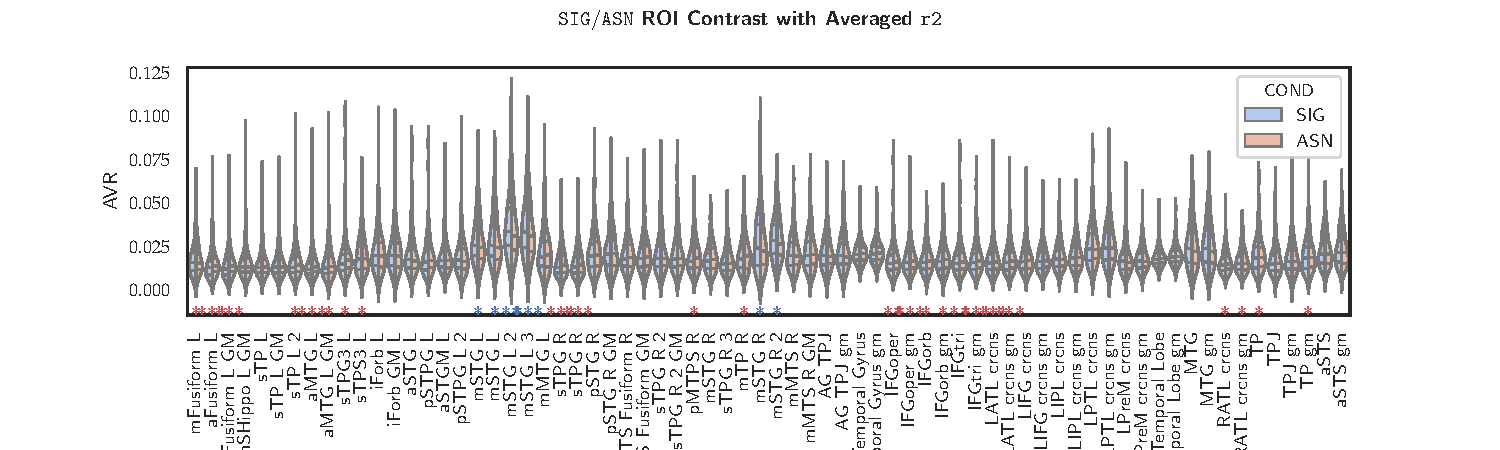
\includegraphics[width=\paperwidth]{Figures/SIG_ASN_ROI.pdf}
    }
    \caption[\code{SIG} \code{ASN} ROI Contrast, Group]{*: 0.05 uncorrected, ***: 0.05 ROI-wise multi-comparison corrected. Red color for \code{ASN}.\\ The average \code{r2} of voxels in a ROI is computed. We select only ROIs with scores>0.02 in either of \code{SIM} and \code{ASN} models. ROIs are of miminum size of 26 voxels (radius of 7 mm). None of the tested ROI reveals a significant mean difference in preference for \code{SIM}. ROIs in left (m,p)STG, l IParietalLobe, lTemporal Lobe respond better to \code{ASN} model.} 
    \label{fig:SIG_ASN_ROI}
\end{figure}

% \subsection{\code{MIX} Nested Model and Contrast}
% [TODO: contrast MIX with SIM, ASN, SIG]

\section{On Behavioral Control}

The correlation between cross-validation session-wise model performances consistently correlates with participants' comprehension question scores in the end of each validation fMRI recording.

\begin{table}
    \centering
    \begin{tabularx}{\textwidth}{L  *{8}{l}}
    \mc{8}{l}{\tabhead{Correlation of Model Performance with Comprehension Question Scores}} \\
    \toprule
    &\mc{2}{c}{\code{SIM}} & \mc{2}{c}{\code{SIG}}& \mc{2}{c}{\code{ASN}} & \mc{2}{c}{\code{MIX}} \\
    \cmidrule{2-3}\cmidrule{4-5}\cmidrule{6-7}\cmidrule{8-9}
    & max & mean & max & mean & max & mean & max & mean \\
    \toprule
    Pearson's r & -.15 & -.17 & -.16 & -.18 & -.09 & -.12 & -.11 & -.14 \\
    p & .0466 & .0221 & .0262 & .0173 & .1329 & .0593 & .4296 & .3893\\
\bottomrule
    
    \end{tabularx}
    \caption[Model Performance and Behavioral Question Score Correlation]{}
    \label{tab:behavioral}
    \end{table}


%\include{Appendices/AppendixC}

\printbibliography[heading=bibintoc]
%% TC:endignore

\end{document}  
